\chapter{Towards Quantifying the Safety of Soft Robots}
\label{chp:safetymetric}

\begin{foreword}
    % Traditionally, most effort in the robotics community has been on achieving safety through computational intelligence, i.e., by constraining motions to remain in a safe set of states, avoid obstacles, and compliant controllers such as impedance control. One of the most interesting and promising aspects of soft robots, on the other hand, is that their embodied intelligence contributes passive compliance to the system. However, in existing literature, the effect on the overall safety of the entire soft robotic system has not been thoroughly investigated or quantified. This lack of safety metric for soft robotics prevents us from considering it during the design process leading to either to badly performing and/or unsafe designs. This chapter proposes a safety metric for soft robots that captures both the embodied intelligence (i.e., the passive behavior) and the computational intelligence (i.e., the controller) of the system, allowing us, for the first time, to investigate quantitatively the effect on each on the overall safety and performance.
    Traditionally, efforts in the robotics community have focused on achieving safety through computational intelligence. This includes constraining motions to remain within safe state sets, avoiding obstacles, and employing compliant controllers such as impedance control. In contrast, one of the most intriguing and promising features of soft robots is their embodied intelligence, which provides passive compliance to the system. Despite this promise, existing literature has yet to thoroughly investigate or quantify the impact of embodied intelligence on the overall safety of soft robotic systems. The absence of a dedicated safety metric for soft robotics hampers the design process, often leading to underperforming or unsafe designs. This chapter introduces a safety metric for soft robots that captures both the embodied intelligence (i.e., the passive behavior) and computational intelligence (e.g., controller) of the system. For the first time, this allows for a quantitative evaluation of their combined effects on system safety and performance.
\end{foreword}

\blfootnote{This chapter is partly based on \faFileTextO~\emph{\textbf{M. Stölzle}*, N. Pagliarani*, F. Stella*, J. Hughes, C. Laschi, D. Rus, M. Cianchetti, C. Della Santina, and G. Zardini (2025). Safe yet Effective Soft Robots via Holistic Co-Design. In Nature Machine Intelligence, \textbf{\emph{In Preparation}}}.

\nth{1}-author contributions: M. Stölzle conceived and implemented the safety metric and all other content presented in this chapter, including the writing, except for Figures \ref{fig:safetymetric:safety_metric_applications} \& \ref{fig:safetymetric:injury_severity_criterion}. 
}

\pagebreak

\begin{abstract}
    % Original version
    % As we work towards integrating robots into human-centric environments, we need to ensure safety while not overly restricting the robot design and/or behavior design. The quest for making robots safer has existed for a long time, with efforts mostly focused on making their control safer and more compliant. Soft robots offer a fundamentally different take on this topic by achieving safety through passive compliance of the entire body. While there has been tremendous research progress in the domain of soft robotics in recent years, ranging from novel actuators to effective model-based control approaches, one of the fundamental promises, safety, has rarely been studied in a principled fashion. In particular, we notice the lack of a quantitative metric to assess how \emph{safe} a soft robot really is. Adding on, we notice that most works take too much of a simplified approach to this topic, equaling safety to material softness. Instead, in reality, the safety of the closed-loop system is influenced by many aspects such as topology, controller, etc, leading to suboptimal soft robot designs that are, for example, too soft to carry practical payloads. Instead, a quantitative safety metric would allow designers to analyze and exploit the safety-vs-performance tradeoff and identify more performant designs while still meeting the necessary safety requirements. In this chapter, we devise requirements a safety metric for soft robots would need to meet. Subsequently, we propose a safety metric that measures the injury severity based on the maximum contact pressure experienced during a collision, as it is already the standard for collaborative robots. Finally, we analyze the safety of continuum soft robots modeled according to the \gls{PCS} parametrization and devise a few simple recommendations for safe soft robot design.
    % short version by ChatGPT
    % Integrating robots into human-centric environments requires ensuring safety without overly restricting the robot's behavior. While soft robotics inherently enhances safety by adding passive body compliance, its core promise—safety—has been largely understudied in a principled manner. Most research equates safety to material softness, overlooking the complex interplay of factors like topology and control systems, which often leads to suboptimal designs that may be too soft to carry practical payloads. A quantitative safety metric could address this issue, enabling designers to balance the trade-off between safety and performance, thus achieving more effective designs while meeting safety requirements. In this chapter, we identify the requirements for a meaningful safety metric for soft robots and propose one based on maximum contact pressure during collisions, consistent with standards for collaborative robots. Using this metric, we analyze the safety of continuum soft robots modeled with the \gls{PCS} parametrization. Finally, we provide recommendations for designing safer soft robots that optimize both performance and safety.
    % longer version by ChatGPT
    As we work toward integrating robots into human-centric environments, it is crucial to ensure safety without overly constraining robot design or behavior. Efforts to enhance robot safety have a long history, primarily focusing on improving control systems to make them safer and more compliant. Soft robots offer a fundamentally different approach to this challenge by achieving safety through the passive compliance of their entire structure. Despite significant advancements in soft robotics over recent years—spanning novel actuators to sophisticated model-based control methods—one of the field’s core promises, safety, has rarely been systematically studied. Notably, there is a lack of a quantitative metric to evaluate how safe a soft robot truly is.
    Moreover, most existing studies oversimplify the concept of safety, equating it to material softness. In reality, the safety of a closed-loop system depends on multiple factors, such as topology and control strategies. This narrow focus often results in suboptimal soft robot designs, such as robots that are too soft to handle practical payloads effectively. A quantitative safety metric would enable designers to evaluate and balance the tradeoff between safety and performance, leading to more optimal designs that meet safety requirements without sacrificing functionality.
    In this chapter, we outline the essential criteria for a safety metric tailored to soft robots. We then propose a metric that assesses injury severity based on the maximum contact pressure during a collision, aligning with established standards for collaborative robots. Finally, we evaluate the safety of continuum soft robots modeled using the \gls{PCS} parametrization and provide practical recommendations for designing safe soft robots.
\end{abstract}

%% Start the actual chapter on a new page.
\newpage

\section{Introduction}
% As already mentioned in Chapter~\ref{chp:introduction}, the soft robotics community frequently emphasizes the "intrinsic safety" and natural compliance of soft robots~\citep{abidi2017intrinsic} - particularly as a differentiating factor from traditional rigid robots and even \glspl{Cobot}~\citep{laschi2014soft, rus2015design, yasa2023overview}.
% However, against scientific best practices, the safety improvement of continuum soft robots compared to rigid manipulators have, to the best of our knowledge, never been quantified. 
% We think that it is crucial for the community to thoroughly validate intrinsic compliance as a very prominent motivation for soft robots in order to justify continued spending into research and development of soft robots~\citep{hawkes2021hard}.
\dropcap{A}s noted in Chapter~\ref{chp:introduction}, the soft robotics community often highlights the “intrinsic safety” and natural compliance of soft robots~\citep{abidi2017intrinsic} as a key advantage over conventional rigid robots and even \glspl{Cobot}~\citep{laschi2014soft, rus2015design, yasa2023overview}. Yet, in contrast to established scientific practices, the safety improvements of continuum soft robots compared to rigid manipulators have not been rigorously quantified. We believe it is essential for the community to validate intrinsic compliance as a fundamental benefit of soft robots, thereby justifying continued investments in their research and development~\citep{hawkes2021hard}.

% Furthermore, as designers currently have no clear guideline for the “right” level of safety, we find that currently they prioritizes an overly soft material for safety.
% Indeed, designers have treated this challenge as a balance between precision and softness, assuming that increasing material compliance inherently improves safety.
% However, \emph{too soft} material choices can compromise the effectiveness of the soft robot, leading to imprecise, oscillatory motions, limited payload capacity, and the inability to exert sufficient forces on the environment~\citep{iida2011soft, cianchetti2013stiff, mazzolai2022roadmap, majidi2014soft, hawkes2017soft}.
% Indeed, we argue that precision vs. softness is an oversimplification, because the safety of soft robots is a function of both body (e.g., morphology) and brain (e.g., control and perception systems).
% Formalizing and quantifying such safety vs. performance tradeoff would enable designers to identify a good balance between the two and maximizing the performance while guaranteeing the necessary safety.
% Indeed, we we anticipate that removing this road-block would lead to more optimal and performant soft robot designs while preserving safety, which is in particular crucial in human-centered environment.
Moreover, in the absence of clear guidelines for determining the optimal level of safety, designers currently tend to favor overly compliant materials. Many treat the challenge as a trade-off between performance/precision and softness, assuming that higher material compliance automatically results in enhanced safety. However, choosing materials that are too soft can undermine the robot’s effectiveness, leading to imprecise or oscillatory motions, reduced payload capacity, and an inability to apply sufficient force to the environment~\citep{iida2011soft, cianchetti2013stiff, mazzolai2022roadmap, majidi2014soft, hawkes2017soft}. We argue that framing the issue as merely a balance between performance and softness oversimplifies the problem, since the safety of soft robots depends on both their body (e.g., morphology) and their brain (e.g., control and perception systems). Formalizing and quantifying this safety–performance trade-off would enable designers to find an optimal balance that maximizes performance while ensuring the necessary safety, a consideration that is particularly critical in human-centered environments.

% Apart from \emph{safety-aware design}, we expect that a safety metric would also be very beneficial for other purposes such as \emph{safety certification} of a soft robotic design or \emph{safety-aware control} where the controller chooses its actions such as that the required safety levels are always met.
% After detailing such potential applications of a safety metric for soft robots in more detail, we devise requirements that a safety metric would need to meet in order to be suitable for the mentioned applications.
% Subsequently, we then propose a new model-based safety metric for soft robots by building an injury criterion on top of the existing ISO norms for collaborative robots~\citep{Isots_15066_2016} while modifying the underlying model to account for the essential characteristics of soft robots, such as the elastic structure that deforms under the influence of internal actuation and external forces, and the potential of collisions along its entire body.
% After modeling the contact model and the collision dynamics between soft robots and humans, we consider analog to ISO/TS 15066:2016~\citep{iso2016collaborative}, the maximum contact pressure experienced during the collision as a proxy for the injury severity. Instead of requiring computationally expensive simulations, we devise a conservative approximation of the collision dynamics, which allows us to determine the maximum contact pressure in closed form.
% Importantly, the proposed safety metric considers the safety of the closed-loop system, which allows us to take the control policy into account when assessing the severity of the injury.
% The safety metric comes in two flavors: \gls{SRISC} computes the injury severity for a known soft robot state, control input, and contact geometry (e.g., point along the soft robot body of contact and collision direction) and is particularly well suited for \emph{safety-aware control} applications. 
% When we want to judge the safety of a soft robot design, we can instead compute the \gls{SRDHC}, which considers all possible contact geometries, soft robot states, etc., within the given operating conditions. We envision the \gls{SRDHC} the metric of choice for \emph{safety-aware design} and \emph{design safety certification}.
Beyond \emph{safety-aware design}, we expect that a comprehensive safety metric will be invaluable for other applications, such as the \emph{safety certification} of soft robotic designs and \emph{safety-aware control}, where the controller adjusts its actions to continuously meet required safety levels. After discussing these potential applications in detail, we establish the requirements a safety metric must satisfy for these purposes. We then introduce a new model-based safety metric for soft robots by extending the injury criterion from the existing ISO norms for collaborative robots~\citep{iso2016collaborative}. Our approach modifies the underlying model to capture key characteristics of soft robots, such as their elastic structures—which deform under internal actuation and external forces—and the possibility of collisions occurring along their entire body. By modeling the contact interactions and collision dynamics between soft robots and humans, and analogously to ISO/TS 15066:2016~\citep{iso2016collaborative}, we use the maximum contact pressure during a collision as a proxy for injury severity. Instead of relying on computationally expensive simulations, we develop a conservative approximation of the collision dynamics that allows us to compute the maximum contact pressure in closed form. Importantly, our safety metric considers the closed-loop system dynamics, incorporating the control policy when assessing injury severity. It is offered in two variants: the \gls{SRISC}, which calculates injury severity for a known soft robot state, control input, and contact geometry (e.g., the specific point of contact and collision direction), making it especially suited for \emph{safety-aware control} applications; and the \gls{SRDHC}, which evaluates safety across all possible contact geometries and robot states within a given operating envelope. We envision the \gls{SRDHC} as the metric of choice for both \emph{safety-aware design} and \emph{design safety certification}.
\section{Towards Quantifying the Safety of Soft Robots}
In the following, we will motivate the need for a quantitative safety metric by showcasing future applications that such a metric would enable.
This will then allow us to define a list of requirements for characteristics that a safety metric needs to exhibit.
Subsequently, we contextualize the topic by reviewing the literature on how safety has been assessed and quantified in the realm of robotics before, where almost all prior work is on the safety of industrial and collaborative rigid robotic manipulators.

\begin{figure}
    \centering
    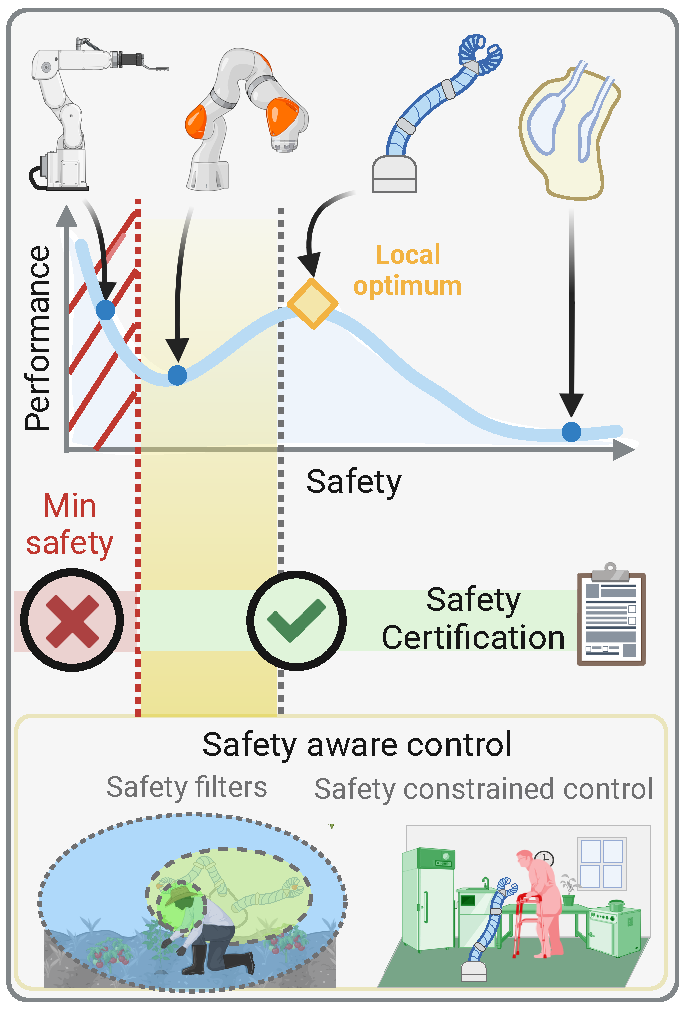
\includegraphics[width=0.5\linewidth]{safetymetric/figures/safety_metric_applications.pdf}
    \caption{Future applications that a quantitative safety metric for soft robots would enable. \textbf{Top:} Here, we showcase how the safety metric could be used for \emph{safety-aware design optimization} and, particularly, for analyzing and exploiting the performance vs. safety tradeoff. Subsequently, the safety metric could be used for certifying a given design as \emph{safe} for the respective application. \textbf{Bottom:} The safety metric could also be used for \emph{safety-aware control} - either by filtering the outputs of the controller without safety guarantees or by explicitly including the safety requirements as constraints during the optimization of the control input sequence (e.g., MPC, Control Barrier Functions).}
    \label{fig:safetymetric:safety_metric_applications}
\end{figure}

\subsection{Potential Applications for a Safety Metric}\label{sub:safetymetric:safety_metric_applications}
% We envision a safety metric for soft robots to unlock a variety of applications that we showcase in Fig.~\ref{fig:safety_metric_applications}, and that can be grouped into the domains of \emph{safety-aware control} and \emph{safety-aware design}.
We envision a safety metric for soft robots that will enable a variety of applications, as illustrated in Fig.~\ref{fig:safetymetric:safety_metric_applications}. These applications can be categorized into two main domains: \emph{safety-aware control} and \emph{safety-aware design}.

% In the domain of \emph{safety-aware control}, we assume the soft robotic design to be given, and we strive to control the actions of the soft robot in such a way that the achieved safety level remains within an acceptable range. We remark that this does not exclude contact or even collision with the environment. Instead, we strive to guarantee that these collisions do not cause any (significant) injuries. Examples include \emph{safety filters}~\cite {bertino2023prescribed} that allow us to use performant control policies that do not explicitly consider the safety constraints (e.g., RL) and still guarantee safety by filtering/saturating the control input. Alternative techniques such as MPC~\citep{hewing2020learning} or Control Barrier Functions~\citep{ames2016control}, which we refer to as \emph{safety-constrained control}, allow us to take the safety constraints directly into account when devising the control input.
In the realm of \emph{safety-aware control}, we assume the soft robotic design is already established and focus on controlling its actions to maintain an acceptable safety level. This approach does not preclude contact or collisions with the environment; rather, it ensures that such interactions do not result in significant injuries. Examples include \emph{safety filters}~\citep{bertino2023prescribed}, which allow the use of high-performance control policies (such as \gls{RL}) that do not explicitly account for safety constraints while still guaranteeing safety by filtering or saturating the control input. Alternative methods like \gls{MPC}~\citep{hewing2020learning} or Control Barrier Functions~\citep{ames2016control}—referred to as \emph{safety-constrained control}—integrate safety constraints directly into the control strategy.

% Another avenue that would be unlocked by a safety metric is \emph{safety-aware design}, which would include assessing an integrated soft robot design for its safety. Specifically, we consider here two subcategories: \emph{safety-aware design optimization} would consider safety when developing/optimizing the soft robot design either by means of inequality constraints (i.e., a minimum safety needs to be guaranteed) or by maximizing safety through the cost function.
% After a design is finalized, \emph{safety certification} would allow manufacturers to certify their product as being sufficiently safe for the respective applications (e.g., healthcare, agri-food, manufacturing, etc.). This is well-aligned with established safety standards for collaborative rigid robots as defined in ISO/TS 15066:2016~\citep{Isots_15066_2016}.
Another promising direction unlocked by a safety metric is \emph{safety-aware design}, which involves evaluating an integrated soft robot design for its safety. We see this as comprising two subcategories: \emph{safety-aware design optimization}, which incorporates safety into the design process either through inequality constraints (ensuring a minimum safety level) or by maximizing safety via the cost function; and \emph{safety certification}, where, after a design is finalized, manufacturers can certify that their product meets the necessary safety standards for specific applications (e.g., healthcare, agri-food, manufacturing, etc.). This approach aligns well with established safety standards for collaborative rigid robots as defined in ISO/TS 15066:2016~\citep{Isots_15066_2016}.

\subsection{Requirements for a Soft Robotic Safety Metric}\label{sub:safetymetric:safety_metric_requirements}
% In the following, we will list some requirements that, in our opinion, a safety metric needs to meet in order to be well suited for the applications listed in Sec.~\ref{sub:safetymetric:safety_metric_applications}.
% First (1), the metric shall consider the dynamics inherent to continuum soft robots and their particular characteristics. For example, one of the main differences between rigid and soft manipulators is that free-moving joints with integrated motors are replaced by an elastic structure that deforms under the influence of internal actuation and external forces. Therefore, any safety metric needs to crucially consider the elastic and inertial characteristics of the soft robot that are generated by the distributed material along its backbone.
% Secondly (2), the safety metric shall consider not just collision at the end-effector but instead anywhere along the body of the soft robot. This is a significant difference to the existing safety metrics for rigid/collaborative robots, which, for simplicity, usually only consider collisions at the end-effector as we would expect there the largest motion velocities~\citep{haddadin2011safe, Isots_15066_2016}. Instead, soft robots exhibit large Cartesian stiffnesses close to their proximal end, thus requiring us to consider the safety of collisions anywhere along the backbone.
% Next, (3) any simplifying assumptions shall lead to a conservative estimate of the achieved safety. For example, soft robot models underlying the safety metric would likely use a finite-dimensional approximation of the continuum shape; instead, in reality, flexible structures such as soft robots exhibit infinite degrees of freedom~\citep{della2023model, armanini2023soft}. Therefore, we would like any safety metric making use of finite-dimensional approximations to underestimate instead of overestimate the safety of the design.
% Fourthly (4), the computation of the safety metric shall be computationally tractable, which is essential for safety-aware control and design applications, where evaluations on the scale of sub-seconds and seconds are necessary.
% Finally, we end with a few desirable characteristics: (5) some applications, such as safety-aware control or safety-aware design, might benefit from the differentiability of the safety metric with respect to design parameters, robot states, and control inputs; (6) ideally, the safety metric shall also consider how \emph{safe} the soft robot's design (e.g., friendly-looking) and behavior (e.g., smooth and predictable movements) is perceived by the user. In addition to user studies, the evaluation of this metric might be assisted by VLMs.
In the following, we outline several requirements that, in our opinion, a safety metric must satisfy to be well-suited for the applications described in Sec.~\ref{sub:safetymetric:safety_metric_applications}. First (1), the metric should account for the dynamics inherent to continuum soft robots and their unique characteristics. For example, a primary difference between rigid and soft manipulators is that free-moving joints with integrated motors are replaced by a compliant structure that deforms under internal actuation and external forces. Consequently, any safety metric must consider the elastic and inertial properties generated by the distributed material along the robot’s backbone.
%
Secondly (2), the safety metric must evaluate collisions occurring anywhere along the soft robot’s body—not just at the end-effector. This represents a significant departure from existing safety metrics for rigid or collaborative robots, which often focus solely on the end-effector due to its typically higher motion velocities~\citep{haddadin2009requirements, haddadin2011safe, Isots_15066_2016}. In contrast, soft robots exhibit high Cartesian stiffness near their proximal end, making it necessary to assess safety along the entire structure.
% 
Next (3), any simplifying assumptions should yield a conservative safety estimate. For instance, while soft robot models used in the metric might employ a finite-dimensional approximation of the continuum shape, in reality, these flexible structures possess infinite degrees of freedom~\citep{della2023model, armanini2023soft}. Therefore, a safety metric based on such approximations should tend to underestimate rather than overestimate the design’s safety.
% 
Fourthly (4), the computation of the safety metric must be tractable, which is essential for safety-aware control and design applications that require evaluations on sub-second to second timescales, respectively.
% 
Finally, we highlight a few desirable characteristics: (5) in applications such as safety-aware control or design, it is advantageous if the safety metric is differentiable with respect to design parameters, robot states, and control inputs; and (6) ideally, the metric should also reflect how “safe” the soft robot’s design (e.g., its friendly appearance) and behavior (e.g., smooth and predictable movements) are perceived by users. In addition to user studies, the evaluation of this metric might be enhanced by leveraging \glspl{VLM}~\citep{touvron2023llama, grattafiori2024llama}.

\subsection{Background on Injury Risk Criteria for Robotic Manipulators}

\begin{itemize}
    \item Give a motivation for why the robotics community strives to quantify safety/injury risk (e.g., optimizing designs and controllers to make them more human-friendly, safety-aware control, etc.).
    \item Give an overview of the trailblazing literature on measuring the injury risk of rigid robots.
    \item Mention the ISO norm that establishes the standards for safe, collaborative robots.
    \item List the existing attempts to assess the safety of soft robots and why they are not sufficient (e.g., too simplistic models, not taking into account the control, lacking a contact model, etc.)
    \item List some of the initial attempts to give designers an idea of which factors influence the safety of soft robots (e.g.,~\citep{abidi2017intrinsic}).
\end{itemize}

\textcolor{red}{Stucture: \begin{enumerate}
    \item Motivation for measuring safety: selecting suitable design, defining constraints that guarantee safety (i.e., ISO norms), and safety-aware control and motion planning
    \item Stress that this is a well-established line of research in (rigid) robotics involving both conceptual and experimental analysis
    \item Modes of impact and injury: constrained vs. unconstrained (human), static vs. dynamic, sharp surfaces, different body parts, etc.~\citep{haddadin2009requirements}
    \item Injurity severity criterias: the first were based on automobile crash models (HIC), but found to be unsuitable as they are calibrated for higher velocities and inertias that are not even relevant for rigid robots. In particular, taking the head acceleration as a injury criteria is not suitable, as not in practice reached, even when robots are moving at 2m/s. Furthermore, it mostly focuses on the question of fatale impacts. Instead, other injury modes, even if not fatal, become relevant as (rigid) robots can still cause bones to break and other significant injuries at their speeds. There exist specialized injury severity criteria inspired by biomechanics for the various body parts. For example, body parts have different contact stiffnesses and injury is (most likely) caused when different thresholds are exceeded (e.g., penetration depth, maximum force, energy density, acceleration). However, it seems that most of them are correlated with the the maximum force experienced during impact and that the maximum force generalizes the best across body parts.
    \item Mention ISO/TS 15066:2016 (Collaborative robots) and ISO/PAS 5672:2023
    \item Safety metrics for soft robots: basically not existing, only~\citep{abidi2017intrinsic}, but only super-simplified beam model. A safety metric is especially important for soft robots as we continuously stress the inherent safety of soft robots, so we also need to be able to quantify it.
\end{enumerate}}

Various aspects have motivated the robotic community to try to assess the safety of our robots~\citep{de2008atlas, van2018spatial}: 
First of all, understanding the important factors influencing safety allows us to make robotic designs and control algorithms safer~\citep{bicchi2004fast, zinn2004new}. 
Secondly, quantifying the injury risk stemming from a robot allows the establishment of minimal safety standards and specifically constraints on the design and actuation that guarantee safe deployment of the robots, as done, for example, in ISO 10218-1:2011~\citep{iso2011robots} for industrial robots and ISO/TS 15066:2016~\citep{Isots_15066_2016} for collaborative robots. This allows the designers and manufacturers of robots to certify that their design is \emph{safe}, which is, in turn, crucial for successful adoption by industrial customers and consumers.
Thirdly, modeling the injury risk of robots and explicitly setting operation constraints that guarantee safety enables safety-aware control~\citep{lacevic2011safety, zanchettin2015safety, mansfeld2018safety}, motion planning~\citep{lacevic2022safe, pupa2024efficient} and also the deployment of safety filters~\citep{hewing2020learning, bertino2023prescribed}.

% Before improving the safety of (collaborative) robots, we first need to understand the important factors influencing the injury risk and be able to compare different robot design w.r.t. to their achieved safety level~\citep{de2008atlas}.
For the reasons mentioned above, quantifying the safety and associated injury risk has been a longstanding research topic, with most effort centered on determining the safety of collaborative rigid robotic manipulators~\citep{zinn2004playing, bicchi2004fast, haddadin2009requirements, mansfeld2018safety}.
\section{A Metric for Quantifying the Safety of Soft Robots}
Thereafter, we propose a quantitative safety metric for \emph{blunt} contacts~\citep{haddadin2011safe} between soft robots and humans that captures the particular characteristics that continuum soft robots exhibit (e.g., elasticity, actuation through their structure, Cosserat rod dynamics, etc.).
Importantly, the presented safety metric fulfills all the mandatory requirements that we laid out previously. % (e.g., based on a soft robotic dynamical model, computationally tractable, differentiable, etc.).
First, we state the necessary background on soft robotic dynamics and contact models. Subsequently, we derive the dynamics of a collision between the continuum soft robot and the human (body part).
Next, we propose two flavors of the safety metric: (i) the \glsxtrfull{SRISC} captures the injury risk for a \emph{given} contact geometry, soft robot state, and actuation sequence. We envision this criterion to be useful for control applications with safety guarantees.
The second flavor, (ii) the \glsxtrfull{SRDHC}, captures the inherent safety of an integrated soft robot design (e.g., also considering the control policy) and leverages the \gls{SRISC} for estimating the maximum injury risk over all possible contact geometries, feasible robot states, and actuation sequences.
Apart from the procedure for formulating this safety metric, one of the key innovations here is that we identify a closed-form solution to the collision dynamics, which renders the computation of the \gls{SRISC} to be computationally tractable.

\subsection{Background on Soft Robot Dynamics and Contact Model}
Following the Cosserat rod theory, we can capture the kinematic behavior of slender structures such as continuum soft robots by considering the deformations of the robot's backbone. As the 1D spatial deformations of this backbone are still an infinite-dimensional problem, the field has developed many methods, such as \gls{PCC}~\citep{webster2010design}, \gls{PCS}~\citep{renda2018discrete}, and \gls{GVS}~\citep{renda2020geometric}, to describe such deformations with a finite number of finite vector of configuration variables $q \in \mathbb{R}^n$. The associated forward kinematic model then allows us to define the geometric positional Jacobian $J_\mathrm{p}(q, s) \in \mathbb{R}^{3 \times n}$, where $s \in (0,L]$ is the backbone abscissa/coordinate and $L$ is the length of the entire continuum structure.
Independent of the specific chosen kinematic model, the \gls{EOM} of a continuum soft robot can often be stated as~\citep{armanini2023soft, della2023model}
\begin{equation}\label{eq:safetymetric:soft_robot_configuration_space_dynamics}
    M(q) \, \ddot{q} + C(q, \dot{q}) \, \dot{q} + \partial_{q} \, \mathcal{U}(q) + D \, \dot{q} = A(q) \, \tau + \tau_\mathrm{c},
\end{equation}
$M(q) \in \mathbb{R}^{n \times n}$ and $C(q, \dot{q}) \in \mathbb{R}^{n \times n}$ considers the inertial and Coriolis effects of the soft robot system, respectively.
$\partial_{q} \, \mathcal{U}(q) \in \mathbb{R}^n$ captures the forces stemming from the potential $\mathcal{U}(q): \mathbb{R}^n \to \mathbb{R}$.
Often times, the potential forces simplify to $\partial_{q} \, \mathcal{U}(q) =  G(q) + K q$, where $G(q) \in \mathbb{R}^{n}$ describes the gravitational forces, and $K \succ 0 \in \mathbb{R}^{n \times n}$ is the stiffness matrix.
Dissipation is integrated through the damping matrix $D \succ 0 \in \mathbb{R}^{n \times n}$.
$\tau(t,q,\dot{q}) \in \mathbb{R}^{m}$ contributes the actuation (determined by a control policy) that acts through the linear map $A(q) \in \mathbb{R}^{n \times m}$ on the generalized coordinates.

The term $\tau_\mathrm{c} \in \mathbb{R}^n$ collects all contributions by external contact forces on the generalized coordinates.
In the following, we will assume that the soft robot is only in contact with the human at one discrete point and that only pure forces are reflected between the bodies during the contact (i.e., no Cartesian torques).
Specifically, we assume that the contact occurs at the backbone abscissa $s_\mathrm{c} \in (0, L]$ and that the contact exhibits a constant surface normal of $n_\mathrm{c} \in \mathcal{S}^3$ which is a unit vector and, with that, $\mathcal{S}^3 = \{ n_\mathrm{c} \in \mathbb{R}^3: \lVert n_\mathrm{c} \rVert_2 = 1 \}$.
We now describe with $\delta_\mathrm{c} > 0$ a penetration between the soft robot and the soft tissue of the human.
Then, the generalized torque acting on the soft robot as a consequence of the contact is given by $\tau_\mathrm{c} = -J^\top(q,s_\mathrm{c}) \, n_\mathrm{c} \, f_\mathrm{c}(\delta_\mathrm{c}, \dot{\delta}_\mathrm{c}) = -J_\mathrm{c}^\top(q, s_\mathrm{c}, n_\mathrm{c}) \, f_\mathrm{c}(\delta_\mathrm{c}, \dot{\delta}_\mathrm{c})$, where $f_\mathrm{c}(\delta_\mathrm{c}, \dot{\delta}_\mathrm{c}) \in \mathbb{R}_{\geq 0}$ is the scalar non-negative contact force.
In the following, we will frequently omit the dependency of symbols, such as $J_\mathrm{c}(q)$, on the $(s_\mathrm{c}, n_\mathrm{c})$ to simplify the notation.
While the formulation that we use in this chapter for formulating the safety metric is compatible with many of the contact models that have been studied in the literature, such as Hunt-Crossley~\citep{hunt1975coefficient, aouaj2021predicting}, Hertz~\citep{johnson1987contact, park2011designing, she2020comparative}, etc., we will mainly focus in the following on a linear spring-damper contact model~\citep{iso2016collaborative, haddadin2009requirements} given by
\begin{equation}
    f_\mathrm{c}(\delta_\mathrm{c}, \dot{\delta}_\mathrm{c}) =
    \begin{cases}
        0 & \delta_\mathrm{c} \leq 0,\\
        k_\mathrm{c} \, \delta_\mathrm{c} + d_\mathrm{c} \, \dot{\delta}_\mathrm{c} & \delta_\mathrm{c} > 0,\\
    \end{cases}
\end{equation}
where $k_\mathrm{c} \in \mathbb{R}_{>0}$ is the contact stiffness and $d_\mathrm{c} \in \mathbb{R}_{\geq 0}$ is the contact damping coefficient.
If we assume the soft robot surface material and the human soft tissue to have spring constants and damping coefficients of $k_\mathrm{R,surf}$, $k_\mathrm{H,st}$ and $d_\mathrm{R}$, $d_\mathrm{H}$, respectively, then we can connect the spring-dampers in series
\begin{equation}
    k_\mathrm{c} = \left (\frac{1}{k_\mathrm{R,surf}} + \frac{1}{k_\mathrm{H,st}} \right )^{-1},
    \qquad
    d_\mathrm{c} = \left (\frac{1}{d_\mathrm{R}} + \frac{1}{d_\mathrm{H}} \right )^{-1}.
\end{equation}
Please note that the effective spring constant of many human body parts is reported in ISO/TS 15066:2016~\citep{iso2016collaborative}.

\subsection{Collision Dynamics}
We now progress towards a formulation of the collision dynamics as motions of the soft robot and the human body part along the contact surface normal $n_\mathrm{c}$.

First, we describe the motion of the contact point of the soft robot with position and velocity $x_\mathrm{R}, \dot{x}_\mathrm{R} \in \mathbb{R}$.
We can project the dynamics of \eqref{eq:safetymetric:soft_robot_configuration_space_dynamics} into this 1D motion through the expression $\dot{x}_\mathrm{R} = J_\mathrm{c} \, \dot{q}$ yielding the form~\citep{khatib1987unified, della2019exact, della2020model, stolzle2024guiding}
\begin{equation}
    \Lambda_\mathrm{c}(q) \, \Ddot{x}_\mathrm{R} + \eta_\mathrm{c}(q,\dot{q}) \, \dot{x}_\mathrm{R} + J_\mathrm{c,M}^{+\top}(q) ( \partial_{q} \, \mathcal{U}(q) + D \dot{q} ) = J_\mathrm{c,M}^{+\top}(q) \, A(q) \, \tau - f_{\mathrm{c}}(\delta_\mathrm{c}, \dot{\delta}_\mathrm{c}),
\end{equation}
where $J_\mathrm{c,M}^{+\top}(q, s_\mathrm{c},n_\mathrm{c}) = M^{-1}J_\mathrm{c}^\top(J_\mathrm{c} M^{-1} J_\mathrm{c}^\top)^{-1} \in \mathbb{R}^{n \times 1}$ is the dynamically consistent pseudo-inverse, $\Lambda_\mathrm{c}(q, s_\mathrm{c},n_\mathrm{c}) = (J_\mathrm{c} \, M^{-1} J_\mathrm{c}^\top)^{-1} \in \mathbb{R}^{1 \times 1}$ is the reflected inertia of the soft robot at the contact point~\citep{haddadin2009requirements, iso2016collaborative}, and $\eta_\mathrm{c}(q,\dot{q},s_\mathrm{c},n_\mathrm{c}) = \Lambda_\mathrm{c}(q) \, (J_\mathrm{c} M^{-1} C - \dot{J}_\mathrm{c}) \in \mathbb{R}^{1 \times n}$ collects the Cartesian Coriolis and centrifugal terms~\citep{khatib1987unified}.
As mentioned already previously, if not explicitly stated otherwise, we will in the following, to simplify the notation, drop the specific dependency on the contact geometry $(s_\mathrm{c}, n_\mathrm{c})$: $J_\mathrm{c,M}^{+\top}(q) = J_\mathrm{c,M}^{+\top}(q,s_\mathrm{c},n_\mathrm{c})$, $\Lambda_\mathrm{c}(q) = \Lambda_\mathrm{c}(q,s_\mathrm{c},n_\mathrm{c})$, etc.

Next, we move towards modeling the behavior of the human body part. In literature, the human body part is usually modeled as a point mass\footnote{Please note that the effective mass of various human body parts is reported in ISO/TS 15066:2016~\citep{iso2016collaborative}.} $m_\mathrm{H}$~\citep{haddadin2011safe, iso2016collaborative} that moves in 1D along the surface normal of the contact with state $(x_\mathrm{H},\dot{x}_\mathrm{H})$. Instead, we take here a conservative approach and assume that the human body is constrained in its motion with velocity $v_\mathrm{H} \in \mathbb{R}$ towards the soft robots (i.e., $m_\mathrm{H} \gg \Lambda(q) \: \forall q$). This represents the \emph{worst case}.
After the coordinate change $\delta_\mathrm{c}(t) = x_\mathrm{R}(t) - x_\mathrm{H}$, $\dot{\delta}_\mathrm{c} = \dot{x}_\mathrm{R}(t) + v_\mathrm{H}$, % where $x^{\mathrm{c}0} \in \mathbb{R}$ is the position of the initial contact, 
where $x_\mathrm{H} \in \mathbb{R}$ is the position of the soft tissue surface, and while only considering the case of contact (i.e., $\delta_\mathrm{c} \geq 0$), the collision dynamics are given by
\begin{equation}
    \Lambda_\mathrm{c}(q) \, \Ddot{\delta}_\mathrm{c} + \eta_\mathrm{c}(q,\dot{q}) \, \dot{\delta}_\mathrm{c} + J_\mathrm{c,M}^{+\top}(q) ( \partial_{q} \, \mathcal{U}(q) + D \dot{q} ) = J_\mathrm{c,M}^{+\top}(q) \, A(q) \, \tau - k_\mathrm{c} \, \delta_\mathrm{c} - d_\mathrm{c} \, \dot{\delta}_\mathrm{c}.
\end{equation}
We are now interested in identifying the maximum force $f_\mathrm{c}(t)$ that occurs during the entire time of the contact.
Therefore, we can neglect any damping forces, such as $d_\mathrm{c} \, \dot{\delta}_\mathrm{c}$ and $D \, \dot{q}$, as they dissipate energy, and, therefore, reduce the maximum contact force.
Furthermore, we assume that the Coriolis effects are sufficiently small and can be neglected as well.
Finally, we assume that the change of configuration during the collision is sufficiently small such that the dynamic matrices can be approximated as constant: 
\begin{equation}\label{eq:safetymetric:constant_reflected_inertia_and_actuation_matrix_definition}
    m_\mathrm{R} = \Lambda_\mathrm{c}(q_{\mathrm{c}}^0) \approx \Lambda_\mathrm{c}(q),
    \qquad
    A_\mathrm{c} = J_\mathrm{c,M}^{+\top}(q_{\mathrm{c}}^0) \, A(q_{\mathrm{c}}^0) \approx J_\mathrm{c,M}^{+\top}(q) \, A(q),
    \quad
    \forall \: t \geq t_\mathrm{c}^0,
\end{equation}
where the $q_{\mathrm{c}}^0$ is the configuration of the robot at the beginning of the contact.
The same assumption also allows us to linearize the potential forces of the soft robot with 
\begin{equation}\label{eq:safetymetric:collision_potential_forces}
    f_{\mathcal{U}} = J_\mathrm{c,M}^{+\top}(q) \, \partial_{q} \, \mathcal{U}(q) \approx \underbrace{J_\mathrm{c,M}^{+\top}(q_{\mathrm{c}}^0) \, \partial_{q} \, \mathcal{U}(q_{\mathrm{c}}^0)}_{f_{\mathcal{U}}^{\mathrm{c}0}} + \underbrace{\frac{\partial}{\partial q} J_\mathrm{c,M}^{+\top}(q) \, \partial_{q} \, \mathcal{U}(q) \Big |_{q=q_{\mathrm{c}}^0} \,  J_\mathrm{c,M}^{+}(q_{\mathrm{c}}^0)}_{k_\mathrm{R}}  \, \delta_\mathrm{c},
\end{equation}
where $k_\mathrm{R} \in \mathbb{R}$ is the local stiffness of the system against small perturbations and $f_{\mathcal{U}}^{\mathrm{c}0}$ are the potential forces present at the start of the contact.
Furthermore, we assume the actuation force to be constant, which can be easily accomplished by conservatively considering the maximum actuation force $f_\tau = \max_t \left | A_\mathrm{c} \, \tau(t) \right |$ that the robot experiences during the collision.
Integrating the stated assumptions into the \gls{EOM} results in the approximated collision dynamics (during contact)
\begin{equation}\label{eq:safetymetric:simplified_collision_dynamics}
    m_\mathrm{R} \, \Ddot{\delta}_\mathrm{c} + (k_\mathrm{R} + k_\mathrm{c}) \, \delta_\mathrm{c} = f_\tau - f_{\mathcal{U}}^{\mathrm{c}0}.
\end{equation}
To avoid computationally expensive simulations of the collision, we identify a closed-form solution to the collision dynamics
\begin{equation}\small\label{eq:safetymetric:collision_dynamics_cfs}
\begin{split}
    \delta_\mathrm{c}(t) =& \: \left (\delta_\mathrm{c}^0-\frac{f_\tau-f_{\mathcal{U}}^{\mathrm{c}0}}{k_\mathrm{R} + k_\mathrm{c}} \right ) \cos \left ( \sqrt{\frac{k_\mathrm{R} + k_\mathrm{c}}{m_\mathrm{R}}} \, t \right ) + \dot{\delta}_\mathrm{c}^0 \sqrt{\frac{m_\mathrm{R}}{k_\mathrm{R} + k_\mathrm{c}}} \, \sin \left ( \sqrt{\frac{k_\mathrm{R} + k_\mathrm{c}}{m_\mathrm{R}}} \, t \right ) + \frac{f_\tau-f_{\mathcal{U}}^{\mathrm{c}0}}{k_\mathrm{R} + k_\mathrm{c}},\\
    \dot{\delta}_\mathrm{c}(t) =& \: -\sqrt{\frac{k_\mathrm{R} + k_\mathrm{c}}{m_\mathrm{R}}} \left (\delta_\mathrm{c}^0 - \frac{f_\tau-f_{\mathcal{U}}^{\mathrm{c}0}}{k_\mathrm{R} + k_\mathrm{c}} \right ) \, \sin \left ( \sqrt{\frac{k_\mathrm{R} + k_\mathrm{c}}{m_\mathrm{R}}} \, t \right ) + \dot{\delta}_\mathrm{c}^0 \, \cos \left ( \sqrt{\frac{k_\mathrm{R} + k_\mathrm{c}}{m_\mathrm{R}}} \, t \right ),
\end{split}
\end{equation}
where we assume without loss of generality that $t_\mathrm{c}^0=0$ at the start of the collision, and $\delta_\mathrm{c}^0$ is the initial penetration depth, although generally $\delta_\mathrm{c}^0 = 0$.
The initial penetration velocity can be computed as a function of the configuration-space velocity as $\dot{\delta}_\mathrm{c}^0 = J_\mathrm{c}(q_{\mathrm{c}}^0) \, \dot{q}_{\mathrm{c}}^0 + v_\mathrm{H}$.

\begin{figure}[h!]
    \centering
    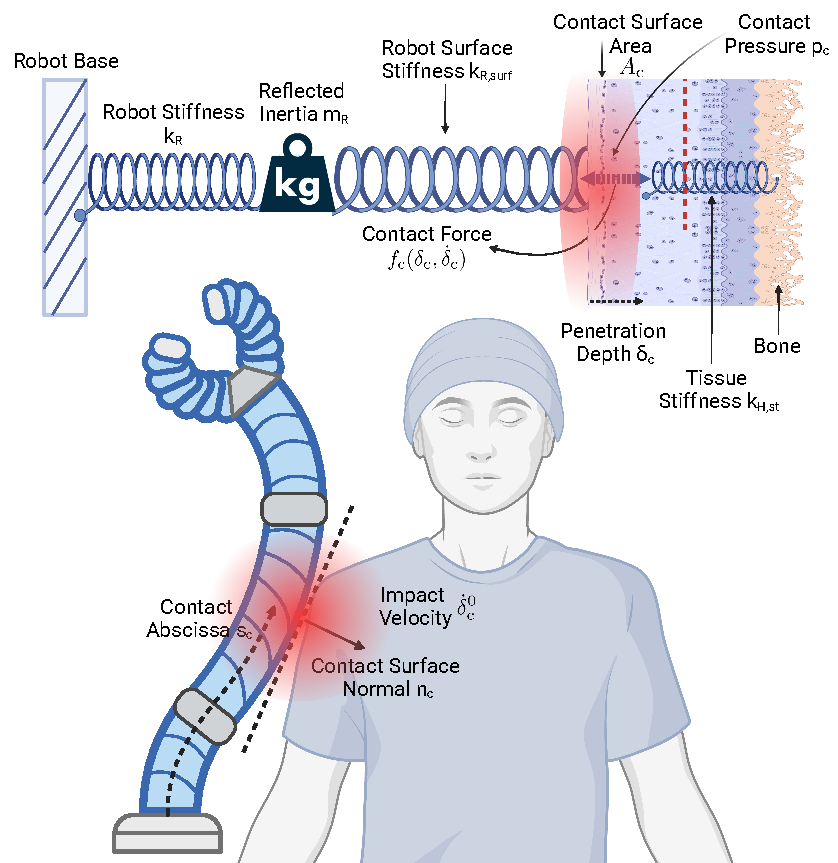
\includegraphics[width=0.65\linewidth]{safetymetric/figures/injury_severity_criterion.pdf}
    \caption{Proposed \glsxtrfull{SRISC} as a safety criterion for soft robots: The maximum contact pressure/stress $\max_t p_\mathrm{c}(t) = \max_t \frac{f_\mathrm{c}(t)}{A_\mathrm{c}}$ experienced during the (potential) collision acts as a proxy for the expected injury risk~\citep{iso2016collaborative}, where $f_\mathrm{c}(t)$ denotes the contact force and $A_\mathrm{c}$ the contact area. For computing $f_\mathrm{c}(t)$, we derive the dynamics of the collision (i.e., the time evolution of the penetration depth $\delta_\mathrm{c}(t)$) by projecting the dynamics of the soft robot onto a 1D Cartesian motion along the contact surface normal. In order to get a conservative estimate of the injury risk, we assume the human body part to be constrained in its motion (i.e., that the inertia of the human body part dominates the reflected inertia of the soft robot $m_\mathrm{R}$).}
    \label{fig:safetymetric:injury_severity_criterion_illustration}
\end{figure}

\subsection{Soft Robot Injury Severity Criterion}
Following the standards established in ISO/TS 15066:2016~\citep{iso2016collaborative}, we consider the maximum contact pressure, also sometimes referred to as stress~\citep{haddadin2009requirements}, experienced during the collision as a proxy for the injury risk. Therefore, we define the \gls{SRISC} for a given tuple $(q_{\mathrm{c}}^0,s_\mathrm{c}, n_\mathrm{c})$ capturing the contact geometry as
\begin{equation}
    \mathrm{SRISC}(q_{\mathrm{c}}^0,\dot{\delta}_\mathrm{c}^0,\tau,s_\mathrm{c},n_\mathrm{c}) = \max_t p_\mathrm{c} = \max_t \frac{f_\mathrm{c}(t)}{A_\mathrm{c}(t)} \leq \frac{\max_t f_\mathrm{c}(t)}{\min_t A_\mathrm{c}(t)} =  \frac{k_\mathrm{c} \max_t \delta_\mathrm{c}(t)}{\min_t A_\mathrm{c}(t)},
\end{equation}
where $p_\mathrm{c}(t)$ is the contact pressure/stress, and $A_\mathrm{c}$ is the contact area. We illustrate the derivation and definition of the \gls{SRISC} in Fig.~\ref{fig:safetymetric:injury_severity_criterion_illustration}.

The closed-form solution to the collision dynamics of \eqref{eq:safetymetric:collision_dynamics_cfs} allows us to upper-bound the maximum contact force $\max_t f_\mathrm{c}(t)$ that is encountered during the collision as
\begin{equation}\label{eq:safetymetric:maximum_contact_force_closed_form}
     \max_{t}f_\mathrm{c}(t) = k_\mathrm{c} \, \left ( \frac{f_\tau-f_{\mathcal{U}}^{\mathrm{c}0}}{k_\mathrm{R} + k_\mathrm{c}} + \sqrt{\left ( \delta_\mathrm{c}^0 - \frac{f_\tau-f_{\mathcal{U}}^{\mathrm{c}0}}{k_\mathrm{R} + k_\mathrm{c}} \right )^2 + \left (\dot{\delta}_\mathrm{c}^0 \right )^2 \frac{m_\mathrm{R}}{k_\mathrm{R} + k_\mathrm{c}} } \right ).
\end{equation}

\begin{figure}[ht]
    \centering
    \subfigure[Penetration depth $\delta_\mathrm{c}(t)$]{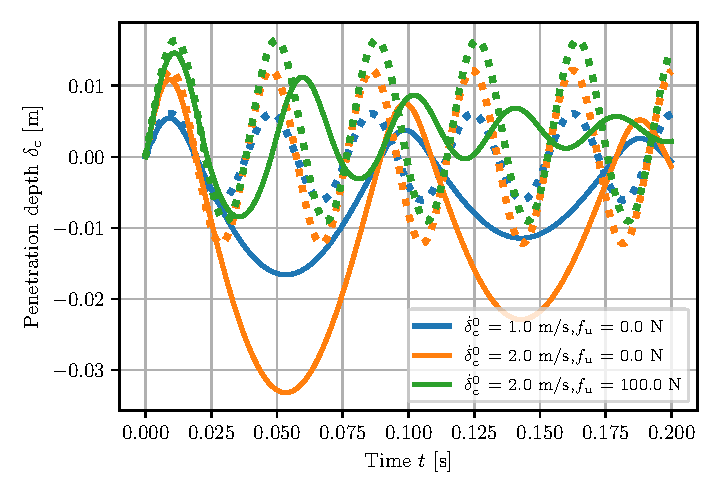
\includegraphics[width=0.49\linewidth, trim={5, 5, 5, 5}]{safetymetric/figures/closed_form_solution_verification/penetration_depth_vs_time.pdf}}
    \subfigure[Penetration velocity $\dot{\delta}_\mathrm{c}(t)$]{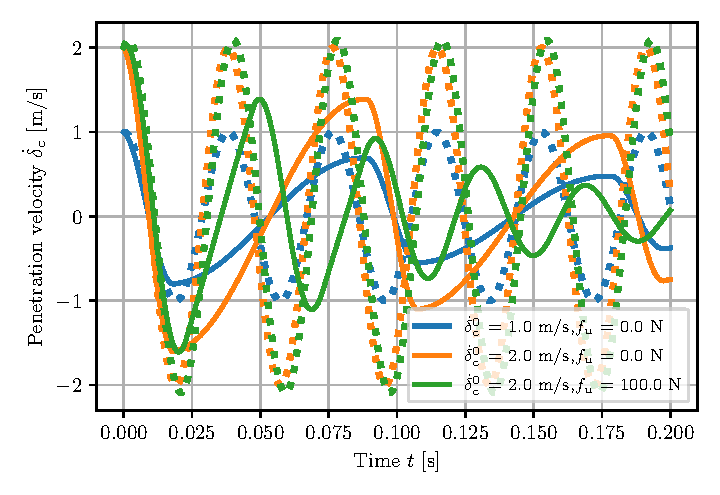
\includegraphics[width=0.49\linewidth, trim={5, 5, 5, 5}]{safetymetric/figures/closed_form_solution_verification/penetration_velocity_vs_time.pdf}}\\
    \subfigure[Contact force $f_\mathrm{c}(t)$]{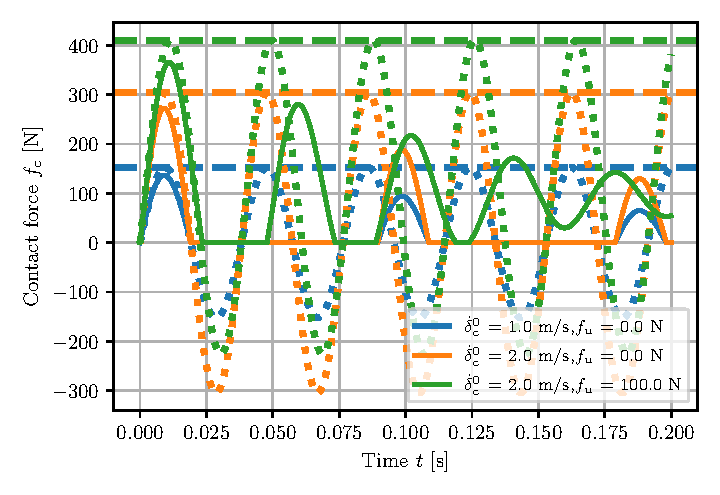
\includegraphics[width=0.5\linewidth, trim={5, 5, 5, 5}]{safetymetric/figures/closed_form_solution_verification/contact_force_vs_time.pdf}}
    \caption{
        Verification of closed-form solution to \eqref{eq:safetymetric:simplified_collision_dynamics}: The solid lines represent numerical integrations of the hybrid dynamics 
        $m_\mathrm{R} \, \Ddot{\delta}_\mathrm{c} + k_\mathrm{R} \, \delta_\mathrm{c} + d_\mathrm{R} \, \dot{\delta}_\mathrm{c} + f_\mathrm{c}(\delta_\mathrm{c}) = f_\tau - f_{\mathcal{U}}^{\mathrm{c}0}$ with $f_\mathrm{c}(\delta_\mathrm{c}) = k_\mathrm{c} \, \delta_\mathrm{c} + d_\mathrm{c} \, \dot{\delta}_\mathrm{c} \: \forall \, \delta_\mathrm{c} > 0$ and $f_\mathrm{c}(\delta_\mathrm{c}) = 0 \: \forall \; \delta_\mathrm{c} \leq 0$. 
        The dotted lines represent the closed-form solution to the time evolution reported in \eqref{eq:safetymetric:collision_dynamics_cfs} based on the dynamics in \eqref{eq:safetymetric:simplified_collision_dynamics} that describe the behavior during the contact phase. The dashed lines represent the (conservative) maximum contact force that could be encountered during the collision as determined by closed-form expression \eqref{eq:safetymetric:maximum_contact_force_closed_form}. 
        As system parameters, we choose $m_\mathrm{R} = \SI{1}{kg}$, $k_\mathrm{R} = \SI{2}{kN \per m}$, $d_\mathrm{R} = \SI{4}{Ns \per m}$, $k_\mathrm{c} = \SI{25}{kN \per m}$, which represents the spring constant of the human chest according to ISO/TS 15066:2016~\citep{iso2016collaborative}, $d_\mathrm{c} = \SI{20}{Ns \per m}$, and $\delta_\mathrm{c}^0 = \SI{0}{m}$.
        Please note that in all case we assume $f_{\mathcal{U}}^{\mathrm{c}0} = 0$ and $v_\mathrm{H} = 0$.
    }
    \label{fig:safetymetric:closed_form_solution_verification}
\end{figure}

We verify and visualize the behavior of the closed-form expression from \eqref{eq:safetymetric:collision_dynamics_cfs} and its upper bound \eqref{eq:safetymetric:maximum_contact_force_closed_form} in Fig.~\ref{fig:safetymetric:closed_form_solution_verification}. It can be clearly seen how \eqref{eq:safetymetric:maximum_contact_force_closed_form} represents a conservative upper bound on the actual contact forces the system experiences if we were to also account for the hybrid nature of the dynamics and the damping of the system.

\begin{figure}[ht!]
    \centering
    \subfigure[Initial deflection $q_\mathrm{c}^0$ vs. Robot stiffness $k_\mathrm{R}$]{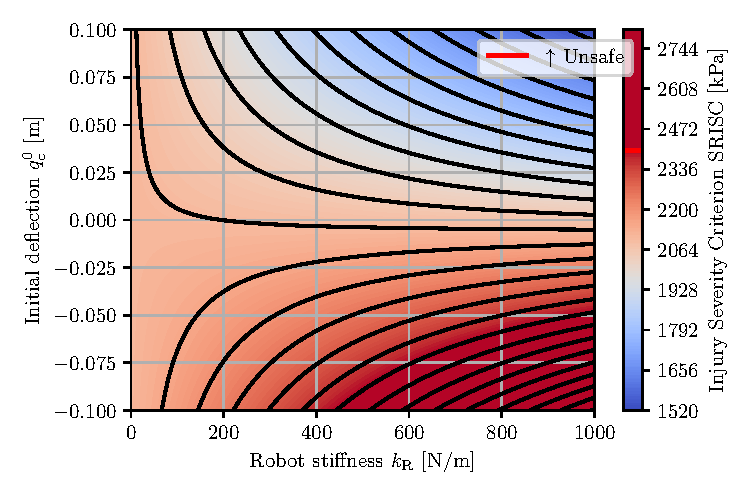
\includegraphics[width=0.49\linewidth, trim={5, 5, 5, 5}]{safetymetric/figures/mass_spring_robot/robot_stiffness_vs_initial_deflection.pdf}\label{fig:safetymetric:mass_spring_robot_characterization:robot_stiffness_vs_initial_deflection}}
    \subfigure[Contact stiffness $k_\mathrm{c}$ vs. robot stiffness $k_\mathrm{R}$]{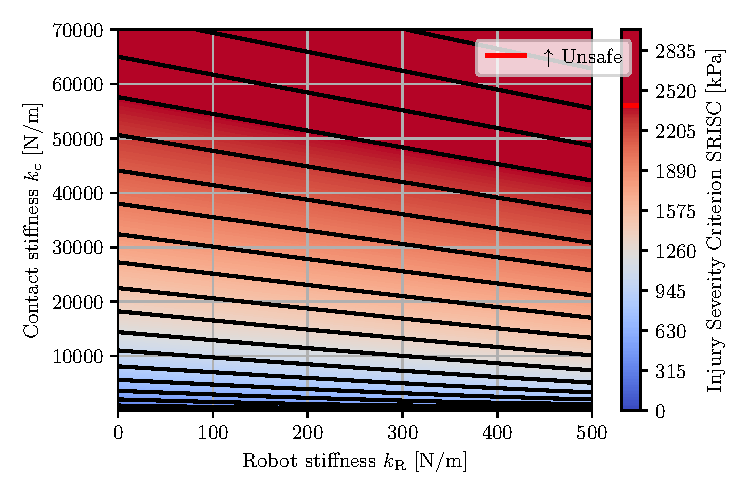
\includegraphics[width=0.49\linewidth, trim={5, 5, 5, 5}]{safetymetric/figures/mass_spring_robot/robot_stiffness_vs_contact_stiffness.pdf}\label{fig:safetymetric:mass_spring_robot_characterization:contact_stiffness_vs_robot_stiffness}}
    \\ \vspace{-0.2cm}
    \subfigure[Initial velocity $\dot{q}_\mathrm{c}^0$ vs. robot mass $m_\mathrm{R}$]{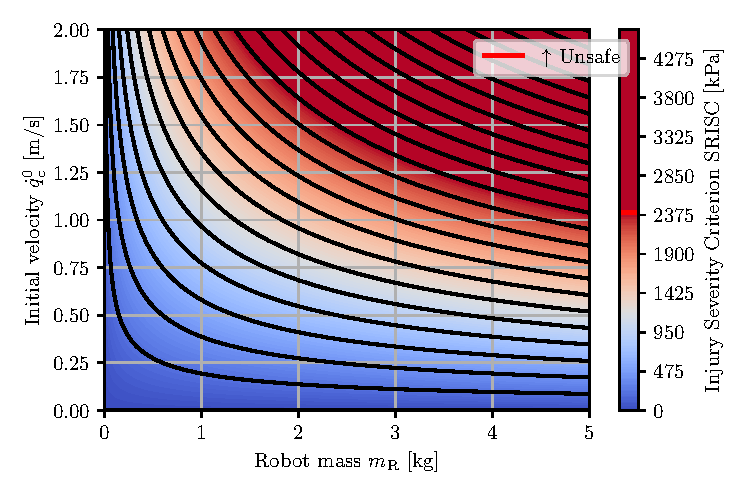
\includegraphics[width=0.49\linewidth, trim={5, 5, 5, 5}]{safetymetric/figures/mass_spring_robot/robot_mass_vs_initial_velocity.pdf}\label{fig:safetymetric:mass_spring_robot_characterization:robot_mass_vs_initial_velocity}}
    \vspace{-0.2cm}
    \caption{Characterization of the \gls{SRISC} on the mass-spring robot example.
        Here, we (closely) consider the collision between the mass-spring robot and the human chest. Therefore, if we conservatively assume the robot surface to be rigid, the spring constant of the contact with the chest is given as $k_\mathrm{c} = k_\mathrm{H} = \SI{25}{kN \per m}$. Furthermore, we assume a contact area of $\SI{1.5}{cm^2}$, an external force of $u=\SI{0}{N}$, and a equilibrium position of $q^0 = \SI{0}{m}$. Finally, according to ISO/TS 15066:2016~\citep{iso2016collaborative}, the maximum acceptable contact pressure/stress in transient conditions is given as $\SI{2400}{kPa}$, which serves as our threshold on the maximum acceptable \gls{SRISC}.
        \textbf{Panel~(a):} Evaluating the influence of robot stiffness $k_\mathrm{R}$ and the deflection of the soft robot at the beginning of the collision $q_\mathrm{c}^0$ on the \gls{SRISC}. We choose $m_\mathrm{R} = \SI{1}{kg}$ and $\dot{q}_\mathrm{c}^0 = \SI{2}{m/s}$.
        \textbf{Panel~(b):} Evaluating the influence of contact stiffness $k_\mathrm{c}$ and the robot stiffness $k_\mathrm{R}$ on the \gls{SRISC}. We choose $m_\mathrm{R} = \SI{1}{kg}$, $q_\mathrm{c}^0 = -\SI{0.1}{m}$, and $\dot{q}_\mathrm{c}^0 = -\SI{1.5}{m/s}$.
        \textbf{Panel~(c):} Evaluating the influence of robot mass $m_\mathrm{R}$ and the robot velocity at the beginning of the collision $\dot{q}_\mathrm{c}^0$ on the \gls{SRISC}. We choose $k_\mathrm{R} = \SI{1}{kN \per m}$ and $q_\mathrm{c}^0 = \SI{0}{m}$.
    }
    \label{fig:safetymetric:mass_spring_robot_characterization}
    \vspace{-0.2cm}
\end{figure}

\subsubsection{Example: Mass-Spring Robot}
First, we consider the most \emph{basic} soft robot - a damped mass-spring system with dynamics 
\begin{equation}
    m_\mathrm{R} \, \ddot{q} + k_\mathrm{R} \, (q-q^0) + d_\mathrm{R} \, \dot{q} = u + f_\mathrm{c},
\end{equation}
where $q \in \mathbb{R}$ and $q^0 \in \mathbb{R}$ is the equilibrium extension. 
Assuming $\delta_\mathrm{c}(t) = q(t)$ (i.e., the robot is in contact with the human when $q \geq 0$) and $v_\mathrm{H} = 0$, the \gls{SRISC} is then given by
\begin{equation}
     \mathrm{SRISC} = \frac{k_\mathrm{c}}{A_\mathrm{c}} \, \left (\frac{u - k_\mathrm{R} (q_{\mathrm{c}}^0 - q^0)}{k_\mathrm{R} + k_\mathrm{c}} + \sqrt{\left ( \frac{u - k_\mathrm{R} (q_{\mathrm{c}}^0 - q^0)}{k_\mathrm{R} + k_\mathrm{c}} \right )^2 + \left (\dot{q}_\mathrm{c}^0 \right )^2 \frac{m_\mathrm{R}}{k_\mathrm{R} + k_\mathrm{c}} } \right ),
\end{equation}
where $q_{\mathrm{c}}^0$ is the mass-spring position at which the collision starts and $\dot{q}_\mathrm{c}^0$ is the associated velocity.

Here, the \gls{SRISC} exhibits the limits
\begin{equation}
    \lim_{k_\mathrm{R} \to 0, u \to 0} \mathrm{SRISC} = \frac{\sqrt{m_\mathrm{R} \, k_\mathrm{c}}}{A_\mathrm{c}} \, \dot{q}_\mathrm{c}^0,
    \qquad
    \lim_{k_\mathrm{R} \to \infty} \mathrm{SRISC} = \frac{k_\mathrm{c}}{A_\mathrm{c}} \, \left ( - (q_{\mathrm{c}}^0 - q^0 ) + \left | q_{\mathrm{c}}^0 - q^0 \right | \right ).
\end{equation}
If $q_{\mathrm{c}}^0 \geq q^0$, which can be interpreted as the spring being in its equilibrium or stretched at the beginning of the collision, then the limit $k_\mathrm{R} \to \infty$ simplifies to $\lim_{k_\mathrm{R} \to \infty} \mathrm{SRISC} = 0$.

We characterize the \gls{SRISC} for this mass-spring robot example in the case of a collision with a human chest and present the results in Fig.~\ref{fig:safetymetric:mass_spring_robot_characterization}. 
Fig.~\ref{fig:safetymetric:mass_spring_robot_characterization:robot_stiffness_vs_initial_deflection} allows us to analyze what influence the robot stiffness has on the \gls{SRISC}: In the limit of $k_\mathrm{R} \to 0$ with $u = 0$, the contact pressure is solely influenced by the robot's initial velocity $\dot{q}_\mathrm{c}^0$, its mass $m_\mathrm{R}$, and the contact stiffness $k_\mathrm{c}$. However, as $k_\mathrm{R} > 0$, we can notice a bifurcation behavior: if the robot is stretched at the beginning of the collision (i.e., $q_\mathrm{c}^0 > 0$), then the contact stress \gls{SRISC} is decreased as $k_\mathrm{R}$ is increased. Oppositely, if the robot is compressed at the beginning of the collision (i.e., $q_\mathrm{c}^0 < 0$), then the contact stress \gls{SRISC} is increased as $k_\mathrm{R}$ is increased.
Fig.~\ref{fig:safetymetric:mass_spring_robot_characterization:contact_stiffness_vs_robot_stiffness} shows, as expected, that increasing the contact stiffness leads to a higher peak contact pressure.
Analog to the known results in the realm of rigid robotics~\citep{haddadin2009requirements, haddadin2013towards}, it can be easily seen in Fig.~\ref{fig:safetymetric:mass_spring_robot_characterization:robot_mass_vs_initial_velocity} how higher velocities and higher robot masses/inertia lead to higher injury severities and safety risks.
This analysis allows us to draw two important takeaways: (1) it is crucial to consider the maximum deformation of the soft robot we would expect to occur during operation to assess its safety, (2) as the robot's stiffness is increased, the \emph{worst-case} injury severity is also increased~\citep{abidi2017intrinsic} - confirming the intuition of how soft robots with their material softness and lower inertia exhibit a more compliant behavior than traditional rigid robots.

\begin{figure}[ht]
    \centering
    \subfigure[Contact backbone coordinate $s_\mathrm{c}$ vs. polar angle $\theta_\mathrm{c}$]{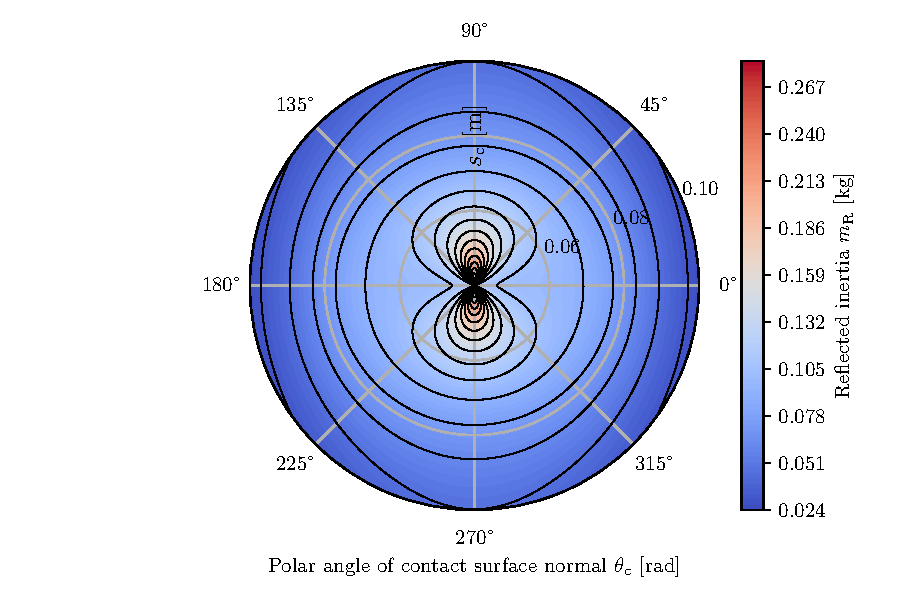
\includegraphics[width=0.43\linewidth, trim={5, 5, 5, 5}]{safetymetric/figures/planar_cs_reflected_inertia_characterization/planar_cs_reflected_inertia_for_theta_vs_s_c_cropped.pdf}}
    \subfigure[Bending strain $\kappa_\mathrm{be}$ vs. axial strain $\sigma_\mathrm{ax}$]{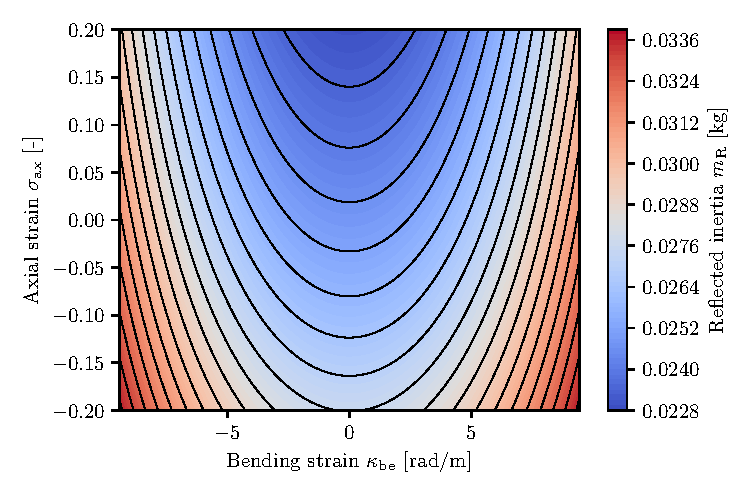
\includegraphics[width=0.56\linewidth, trim={5, 5, 5, 5}]{safetymetric/figures/planar_cs_reflected_inertia_characterization/planar_cs_reflected_inertia_for_kappa_be_vs_sigma_ax.pdf}}
    \caption{Characterization of the reflected inertia, also called effective mass~\citep{haddadin2009requirements, kirschner2021notion}, on the example of a planar \gls{CS} soft robot. 
    \textbf{Left:} Variation of the collision backbone coordinate $s_\mathrm{c}$ against the polar angle of contact $\theta_\mathrm{c}$, where $\theta_\mathrm{c} = 0$ corresponds to a perpendicular collision with the backbone and $n_\mathrm{c} = (1, 0)$ and $\theta_\mathrm{c} = \frac{\pi}{2}$ relates to a parallel collision with the robot backbone and $n_\mathrm{c} = (0,1)$. We assume here a soft robot in its equilibrium configuration (i.e., $q = 0_3$).
    \textbf{Right:} Variation of the bending strain $\kappa_\mathrm{be}$ and the axial strain $\sigma_\mathrm{ax}$ for a perpendicular collision ($n_\mathrm{c} = (0,1)$) at the distal end of the robot ($s_\mathrm{c} = \SI{0.1}{m}$).
    }
    \label{fig:safetymetric:planar_cs_reflected_inertia_characterization}
    \vspace{-0.2cm}
\end{figure}

\begin{figure}[ht]
    \centering
    \subfigure[Contact backbone coordinate $s_\mathrm{c}$ vs. polar angle $\theta_\mathrm{c}$]{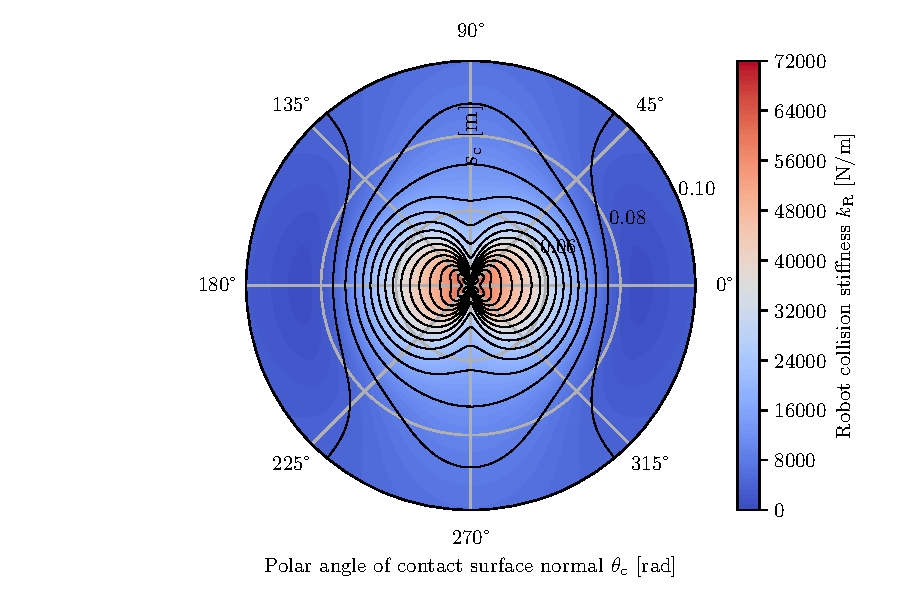
\includegraphics[width=0.49\linewidth]{safetymetric/figures/planar_cs_robot_collision_stiffness_characterization/planar_cs_robot_collision_stiffness_for_theta_c_vs_s_c_cropped.pdf}\label{fig:safetymetric:planar_cs_robot_collision_stiffness_characterization:theta_c_vs_s_c}}
    \subfigure[Bending strain $\kappa_\mathrm{be}$ vs. contact polar angle $\theta_\mathrm{c}$]{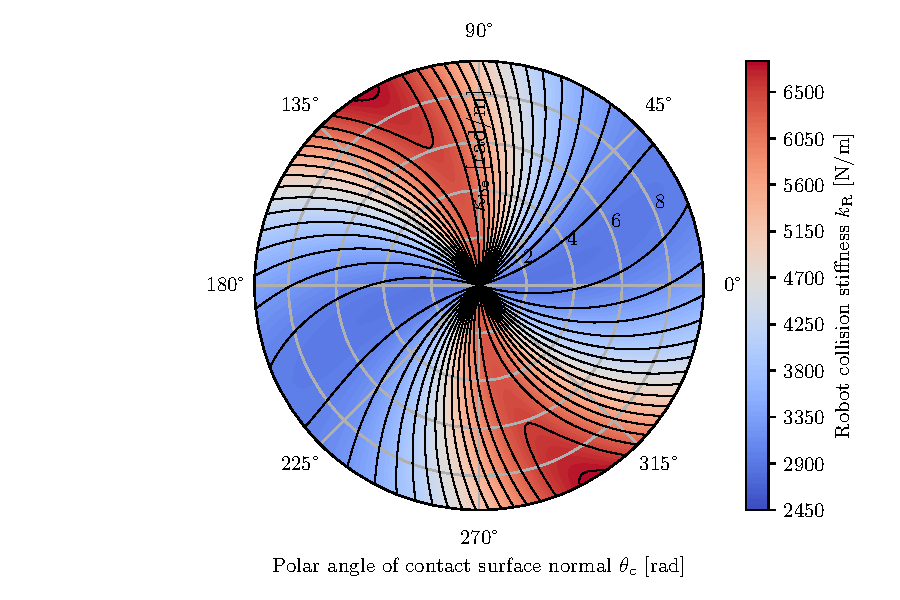
\includegraphics[width=0.49\linewidth]{safetymetric/figures/planar_cs_robot_collision_stiffness_characterization/planar_cs_robot_collision_stiffness_for_theta_c_vs_kappa_be_cropped.pdf}\label{fig:safetymetric:planar_cs_robot_collision_stiffness_characterization:theta_c_vs_kappa_be}}
    \caption{Characterization of the local robot collision stiffness $k_\mathrm{R}$ vs. polar angle $\theta_\mathrm{c}$ on the example of a planar \gls{CS} soft robot.
    \textbf{Left:} Variation of the collision backbone coordinate $s_\mathrm{c}$ against the polar angle of contact $\theta_\mathrm{c}$, where $\theta_\mathrm{c} = 0$ corresponds to a perpendicular collision with the backbone and $n_\mathrm{c} = (1, 0)$ and $\theta_\mathrm{c} = \frac{\pi}{2}$ relates to a parallel collision with the robot backbone and $n_\mathrm{c} = (0,1)$. We assume here a soft robot in its equilibrium configuration (i.e., $q = 0_3$).
    \textbf{Right:} Variation of the bending strain $\kappa_\mathrm{be}$ against the polar angle of contact $\theta_\mathrm{c}$ at the distal end of the robot ($s_\mathrm{c} = \SI{0.1}{m}$).
    }
    \label{fig:safetymetric:planar_cs_robot_collision_stiffness_characterization}
\end{figure}

\subsubsection{Example: Planar Piecewise Constant Strain Robot}
% 1 Figure giving an example how the contact location influences the injury severity.
% \begin{itemize}
%     \item Variation of injury severity for various contact geometries (e.g., various locations along the backbone, various contact surface normal) and configurations.
%     \item Variation across model discretization granularity.
% \end{itemize}

We now consider a planar $N$ segment \gls{PCS} robot, as introduced in Chapter~\ref{chp:background}. Here, the configuration of the $i$th segment is characterized by its spatially constant strain $\xi_i = \begin{bmatrix}
    \kappa_{\mathrm{be},i} & \sigma_{\mathrm{sh},i} & \sigma_{\mathrm{ax},i}
\end{bmatrix}^\top$, where $\kappa_{\mathrm{be},i}$ is the bending, $\sigma_{\mathrm{sh},i}$ the shear, and $\sigma_{\mathrm{ax},i}$ the axial/elongation strain~\citep{renda2018discrete}.
The collision dynamics are then given as
\begin{equation}
    \Lambda_\mathrm{c}(q) \, \Ddot{\delta}_\mathrm{c} + \eta_\mathrm{c}(q,\dot{q}) \, \dot{\delta}_\mathrm{c} + J_\mathrm{c,M}^{+\top}(q) ( G(q) + S \, q + D \dot{q} ) = J_\mathrm{c,M}^{+\top}(q) \, A(q) \, \tau - k_\mathrm{c} \, \delta_\mathrm{c} - d_\mathrm{c} \, \dot{\delta}_\mathrm{c},
\end{equation}
where $S \in \mathbb{R}^{3N \times 3N}$ is the linear stiffness of the robot, $G(q) \in \mathbb{R}^{3N}$ captures the gravitational forces, and $\tau \in \mathbb{R}^m$ represents the actuator forces.
We build the JAX~\citep{jax2018github} implementation of these dynamics on the \emph{JSRM}\footnote{\url{https://github.com/tud-phi/jax-soft-robot-modelling}} package~\citep{stolzle2024experimental}.

As we have seen in the previous example of the mass-spring robot, two of the variables that have the largest impact on the \gls{SRISC} are the reflected inertia $m_\mathrm{R}$, as defined in
\eqref{eq:safetymetric:constant_reflected_inertia_and_actuation_matrix_definition}, and the local soft robot stiffness in the collision direction $k_\mathrm{R}$, as defined in \eqref{eq:safetymetric:collision_potential_forces}.
Therefore, we present in Figures \ref{fig:safetymetric:planar_cs_reflected_inertia_characterization} \& \ref{fig:safetymetric:planar_cs_robot_collision_stiffness_characterization} a characterization of the reflected inertia $m_\mathrm{R}$ and the local robot stiffness $k_\mathrm{R}$, respectively.
In both cases, we consider a planar \gls{CS} segment (i.e., $N=1$) that has a length of $\SI{0.1}{m}$, a radius of \SI{0.02}{m}, a material density of \SI{1070}{kg \per m^3}, an elastic modulus of $E=\SI{0.5}{MPa}$ and a shear modulus of $G=\SI{0.2}{MPa}$.
The results show that the reflected inertia is highest at the proximal end of the robot/segment (i.e., $s_\mathrm{c} \to 0$) and for collisions that are parallel to the backbone, which, for our definition of our coordinate system with the soft robot in its straight configuration aligned with the y-axis, means that $\theta_\mathrm{c} = \frac{\pi}{2} + \pi \, n$ and $n_\mathrm{c} = \begin{bmatrix}
    0 & \pm 1
\end{bmatrix}^\top$. Furthermore, when considering perpendicular collisions with the backbone, the inertia increases with the bending strain and a compressed backbone (i.e., an increase in mass density).
Concerning the robot collision stiffness, we find that it is highest at the proximal end of the soft robot. At the distal end, we identify larger stiffnesses for parallel collisions, although the exact characteristics will depend on the choice of backbone radius/second moment of area. With increased bending strain, the polar angle with the highest stiffness will also change, as seen in Fig.~\ref{fig:safetymetric:planar_cs_robot_collision_stiffness_characterization:theta_c_vs_kappa_be}.

\begin{figure}[ht!]
    \centering
    \subfigure[Bending strain velocity $\dot{\kappa}_\mathrm{be}$ vs. mass density $\rho$]{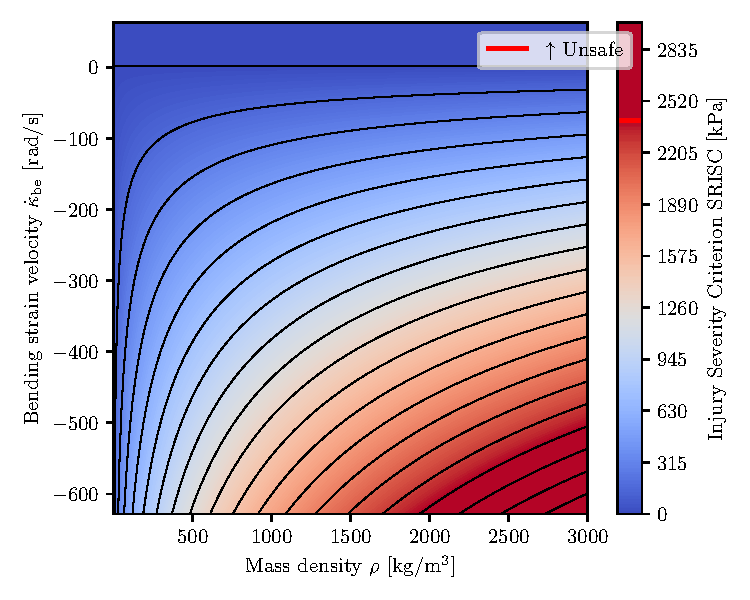
\includegraphics[width=0.49\linewidth]{safetymetric/figures/planar_cs_injury_severity_criterion/planar_cs_isc_for_bending_strain_velocity_vs_mass_density.pdf}\label{fig:safetymetric:planar_cs_injury_severity_criterion:bending_strain_velocity_vs_mass_density}}
    \subfigure[Robot length $L$ vs. backbone coordinate $s_\mathrm{c}$]{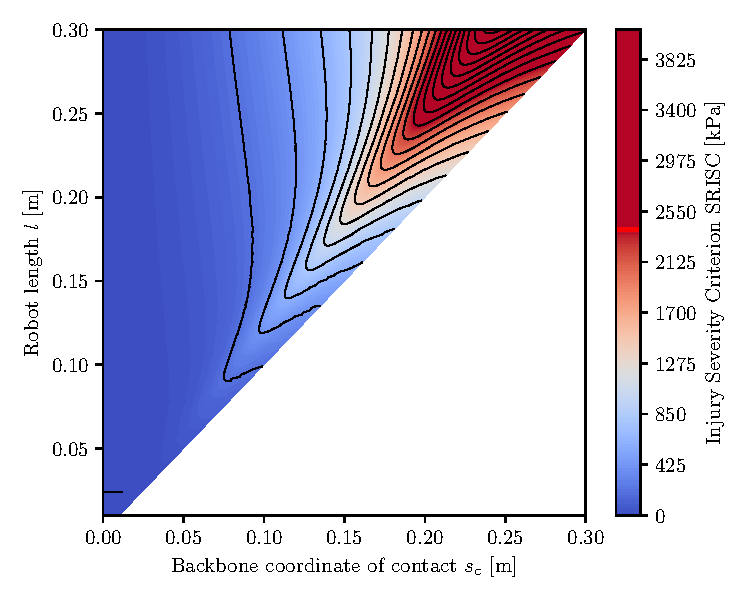
\includegraphics[width=0.49\linewidth]{safetymetric/figures/planar_cs_injury_severity_criterion/planar_cs_isc_robot_length_vs_s_c.pdf}\label{fig:safetymetric:planar_cs_injury_severity_criterion:robot_length_vs_s_c}}
    \\
    \subfigure[Contact backbone coordinate $s_\mathrm{c}$ vs. polar angle $\theta_\mathrm{c}$]{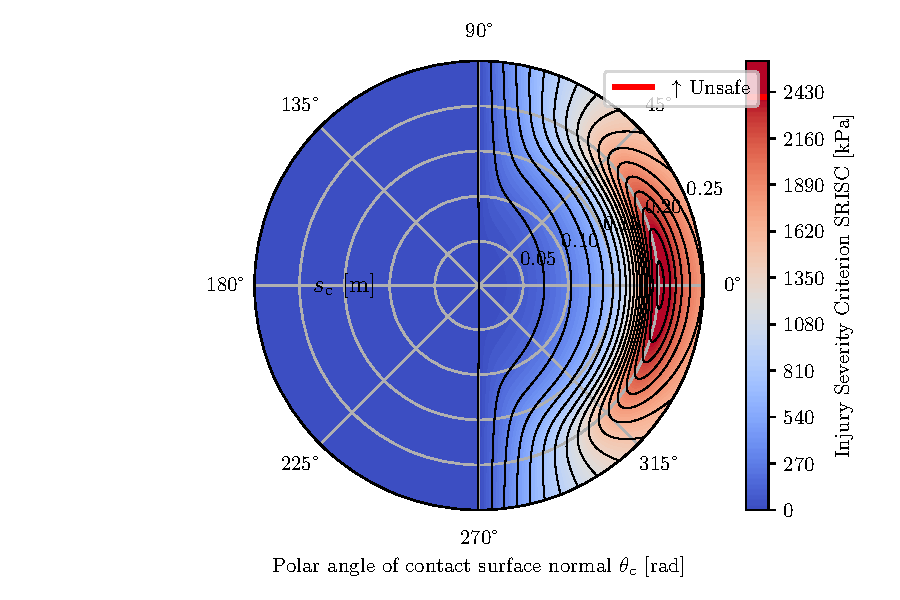
\includegraphics[width=0.49\linewidth]{safetymetric/figures/planar_cs_injury_severity_criterion/planar_cs_isc_for_theta_c_vs_s_c_cropped.pdf}\label{fig:safetymetric:planar_cs_injury_severity_criterion:theta_c_vs_s_c}}
    \subfigure[Bending strain $\kappa_\mathrm{be}$ vs. polar angle $\theta_\mathrm{c}$]{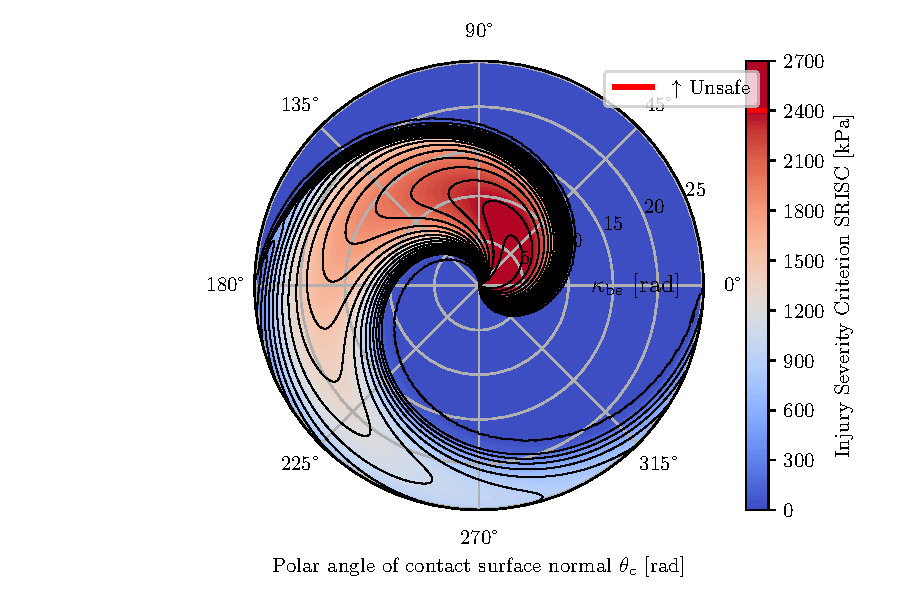
\includegraphics[width=0.49\linewidth]{safetymetric/figures/planar_cs_injury_severity_criterion/planar_cs_isc_for_theta_c_vs_kappa_be_cropped.pdf}\label{fig:safetymetric:planar_cs_injury_severity_criterion:theta_c_vs_kappa_be}}
    \caption{Characterization of the \gls{SRISC} on a planar \gls{CS} robot.
    \textbf{Panel~(a):} Variation of the robot's mass density $\rho$ and the bending strain velocity $\dot{\kappa}_\mathrm{be}$. We assume a perpendicular collision ($n_\mathrm{c} = (1,0)$) at the tip of the segment ($s_\mathrm{c} = \SI{0.25}{m}$).
    \textbf{Panel~(b):} Variation of the total robot length $L$ and the backbone coordinate $s_\mathrm{c}$ where the collision occurs. We assume a perpendicular collision ($n_\mathrm{c} = (1,0)$) with a soft robot in its equilibrium configuration (i.e., $q=0_3$).
    \textbf{Panel~(c):} Variation of the backbone coordinate $s_\mathrm{c}$ against the polar angle $\theta_\mathrm{c}$ of the contact surface where the collision occurs. Here, $\theta_\mathrm{c} = 0$ corresponds to a surface normal of $n_\mathrm{c} = (1,0)$ and $\theta_\mathrm{c} = \frac{\pi}{2}$ to $n_\mathrm{c} = (0,1)$. The soft robot is assumed to be in its equilibrium configuration (i.e., $q=0_3$).
    \textbf{Panel~(d):} Variation of the bending strain $\kappa_\mathrm{be}$ against the polar angle $\theta_\mathrm{c}$ of the contact surface where the collision occurs. We assume a collision with the distal end of the soft robot (i.e., $s_\mathrm{c} = \SI{0.25}{m}$).
    }
    \label{fig:safetymetric:planar_cs_injury_severity_criterion}
\end{figure}

In Fig.~\ref{fig:safetymetric:planar_cs_injury_severity_criterion}, we characterize the behavior of the \gls{SRISC} on the case of a planar \gls{CS} soft robot with a nominal robot length $L = \SI{0.25}{m}$, a backbone radius of $R = \SI{0.02}{m}$, a nominal mass density of $\rho = \SI{1070}{kg \per m^3}$, an elastic modulus of $E = \SI{0.5}{MPa}$, a shear modulus of $G = \SI{0.2}{MPa}$, a contact area of $A_\mathrm{c} = \SI{1.5}{cm^2}$, the spring constant of the human chest $k_\mathrm{H,st} = \SI{25}{kN \per m}$, and a soft robot surface material stiffness of $k_{\mathrm{R,surf}} = \SI{7.5}{kN \per m}$.
In all cases, we set the external forcing to $f_\tau = 0_3$, consider the human to be stationary and constrained with $v_\mathrm{H} = \SI{0}{m \per s}$, and assume a maximum threshold of \SI{2400}{kPa} on the \gls{SRISC}, which mirrors the maximum transient contact stress that is acceptable for collisions with the chest sternum according to ISO/TS 15066:2016~\citep{iso2016collaborative}.
% In Fig.~\ref{fig:safetymetric:planar_cs_injury_severity_criterion:bending_strain_velocity_vs_mass_density}, we can observe that, as expected, the maximum contact stress, and with that, the \gls{SRISC}, increases with mass density and a larger bending velocity in the direction of the collision.
% The results shown in Fig.~\ref{fig:safetymetric:planar_cs_injury_severity_criterion:robot_length_vs_s_c} are very interesting: while the \gls{SRISC} increases with an increased length of the segment, which is not too unexpected as longer soft robots exhibit larger Cartesian space velocities for the same strain-space velocities, we observe the the maximum contract stress is usually not at the tip of the distal end of the robot, but instead at at roughly \SI{75}{\percent} of its length. We hypothesize that the underlying reason is that some quantities, such as stiffness and reflected inertia, are at their maximum at the proximal end, while other quantities - in particular the Cartesian velocity - are at their maximum and the distal end leading the global maximum of the \gls{SRISC} to be in between proximal and distal end.
% Fig.~\ref{fig:safetymetric:planar_cs_injury_severity_criterion:theta_c_vs_s_c} exhibits the same characteristics while the polar angle with the maximum contact stress will always depend on the velocities and actuation that are applied to the soft robot.
% Finally, we observe in Fig.~\ref{fig:safetymetric:planar_cs_injury_severity_criterion:theta_c_vs_kappa_be} the maximum \gls{SRISC} to be at a straight backbone configuration with the \gls{SRISC} decreasing with an increased bending strain.
In Fig.\ref{fig:safetymetric:planar_cs_injury_severity_criterion:bending_strain_velocity_vs_mass_density}, we see that, as expected, the maximum contact stress—and therefore the \gls{SRISC}—rises with increased mass density and higher bending velocity in the collision direction. The results in Fig.~\ref{fig:safetymetric:planar_cs_injury_severity_criterion:robot_length_vs_s_c} are particularly intriguing: while the \gls{SRISC} increases with longer segment lengths—as longer soft robots exhibit higher Cartesian velocities for the same strain-space velocities—the maximum contact stress is typically not located at the very tip of the distal end but rather around \SI{75}{\percent} of the robot’s length. We hypothesize that this occurs because certain factors, such as stiffness and reflected inertia, peak at the proximal end, whereas others—especially Cartesian velocity—are maximized at the distal end, leading to an overall maximum \gls{SRISC} somewhere between the two. Similarly, Fig.~\ref{fig:safetymetric:planar_cs_injury_severity_criterion:theta_c_vs_s_c} displays analogous behavior, with the polar angle corresponding to the maximum contact stress varying based on the velocities and actuation applied to the soft robot. Finally, Fig.~\ref{fig:safetymetric:planar_cs_injury_severity_criterion:theta_c_vs_kappa_be} shows that the maximum \gls{SRISC} occurs at a straight backbone configuration, with the maximum \gls{SRISC} decreasing as bending strain increases.

\subsubsection{Example: Integrating a Control Policy}
% alternative heading: \subsection{Influence of Control Policy}
An important question when analyzing the safety of a closed-loop soft robotic system is what influence the control policy has on the \gls{SRISC}.
First, we consider a case where the behavior of the control policy $\tau(q,\dot{q})$ cannot be bounded or even inspected, such as it would be the case for controllers that contain integral terms or for many RL-based control policies.
In this case, access to actuation bounds $[\tau_\mathrm{min}, \tau_\mathrm{max}]$ provides us with the injury risk in the \emph{worst case scenario}.

Next, we consider the example of a \emph{PD+Feedforward}-like control structure that is relevant for many control policies that involve feedforward and/or feedback terms.
Specifically, we consider a fully-actuated setting (i.e., $n=m$) with an identity actuation matrix $A(q) = \mathbb{I}^n$.
Then, a regulator $\tau(q,\dot{q}) = \partial_{q} \, \mathcal{U}( q^\mathrm{d}) + K_\mathrm{p} \, (q^\mathrm{d}-q) - K_\mathrm{d} \, \dot{q}$ drives the system towards the setpoint $q^\mathrm{d}$~\citep{della2023model} and establishes the closed-loop dynamics
\begin{equation}
    M(q) \, \ddot{q} + C(q, \dot{q}) \, \dot{q} + \partial_{q} \, \mathcal{U}(q) + K_\mathrm{p} \, q + (D+K_\mathrm{d}) \, \dot{q} = \partial_{q} \, \mathcal{U}( q^\mathrm{d}) + K_\mathrm{p} \, q^\mathrm{d} + \tau_\mathrm{c},
\end{equation}
where $K_\mathrm{p}, K_\mathrm{d} \in \mathbb{R}^{n \times n}$ are the proportional and derivative feedback gains, respectively.
When re-formulating the simplified collision dynamics of \eqref{eq:safetymetric:simplified_collision_dynamics}, 
\begin{equation}
    m_\mathrm{R} \, \Ddot{\delta}_\mathrm{c} + (k_\mathrm{R} + k_\mathrm{c}) \, \delta_\mathrm{c} = J_\mathrm{c,M}^{+}(q_{\mathrm{c}}^0) \, (\partial_{q} \, \mathcal{U}(q^\mathrm{d}) +  K_\mathrm{p} \, q^\mathrm{d} - \partial_{q} \, \mathcal{U}(q_{\mathrm{c}}^0)).
\end{equation}
We notice that the feedforward control term acts through a constant force on the oscillatory system.
The proportional feedback term increases the local stiffness of the robot: $k_\mathrm{R} = \frac{\partial}{\partial q} J_\mathrm{c,M}^{+\top}(q) \, \left ( \partial_{q} \, \mathcal{U}(q) + K_\mathrm{p} \, q \right )\Big |_{q=q_{\mathrm{c}}^0} \,  J_\mathrm{c,M}^{+}(q_{\mathrm{c}}^0)$.
This analysis agrees with similar results known in literature~\citep{della2017controlling}.

\subsection{Soft Robot Design Hazardousness Criterion}
As presented in Fig.~\ref{fig:safetymetric:safety_metric_applications}, one application of a soft robotic safety metric would be to answer the question "\emph{How safe is this proposed soft robot design?}". The \gls{SRISC} on its own is not sufficient to answer this question as it relies on a knowledge of the soft robot state at the beginning of the collision $(q_{\mathrm{c}}^0, \dot{q}_{\mathrm{c}}^0)$, and the contact geometry $(s_\mathrm{c},n_\mathrm{c})$.
Therefore, we define the \gls{SRDHC} as the maximum injury severity that can be imposed by the soft robot over all feasible soft robot states, all possible contact geometries, and actuation sequences~\citep{wassink2007towards}
\begin{equation}
\begin{split}
    \mathrm{SRDHC} =& \: \max_{q \in \mathcal{Q}} \max_{\dot{\delta}_\mathrm{c}^0 \in [0,\dot{\delta}_\mathrm{c}^\mathrm{max}]} \max_{\tau \in [\tau_\mathrm{min}, \tau_\mathrm{max}]} \max_{s_\mathrm{c} \in (0,L]} \max_{n_\mathrm{c} \in \mathcal{S}^3} \mathrm{SRISC}(q_{\mathrm{c}}^0,\dot{\delta}_\mathrm{c}^0,\tau,s_\mathrm{c},n_\mathrm{c}),\\
    \leq& \: \max_{q \in \mathcal{Q}} \max_{s_\mathrm{c} \in (0,L]} \max_{n_\mathrm{c} \in \mathcal{S}^3} \mathrm{SRISC}(q_{\mathrm{c}}^0,\dot{\delta}_\mathrm{c}^\mathrm{max},\lVert \tau_\mathrm{max} \rVert_2,s_\mathrm{c},n_\mathrm{c}),
\end{split}
\end{equation}
where $\mathcal{Q}$ is the set of feasible soft robot configurations.
To make this optimization more tractable, we can leverage the stated upper bound with $\dot{\delta}_\mathrm{c}^\mathrm{max} = \lVert J_\mathrm{c} \rVert_2 \, \lVert \dot{q}_\mathrm{max} \rVert_2 + v_\mathrm{H}$
and $f_\tau^\mathrm{max} = \lVert A_\mathrm{c} \rVert_2 \, \lVert \max(|\tau_\mathrm{min}|,|\tau_\mathrm{max}|) \rVert_2$.
We note that the maximum value of $\dot{q}_\mathrm{max}$ that the robot can achieve autonomously is, in practice, often given by certain actuator characteristics (e.g., maximum servo velocity for tendon-driven actuation).

% We performed a preliminary investigation on the effect of the discretization on the estimated safety - and, in particular, the \gls{SRDHC}.
% The initial results reported in Fig.~\ref{fig:safetymetric:planar_pcs_design_hazardousness_criterion_discretization} show that approximating the soft robot with one or a few segments represents a conservative estimate of the actual safety - i.e., an overestimation of the injury severity. The underlying reason behind this behavior is that the actual soft robots can deform in infinite-dimensional space, while the approximation via the planar \gls{PCS} model limits the deformation modes and, with that, often increases the stiffness upon local contact. By increasing the discretization of the kinematic model underlying the safety metric, we can account for more deformation modes, and with that, reduce the overestimate of the injury severity.
We conducted a study to assess how discretization affects the estimated safety, with a particular focus on the \gls{SRDHC}. The initial results shown in Fig.~\ref{fig:safetymetric:planar_pcs_design_hazardousness_criterion_discretization} for varying the number of \gls{PCS} segments while keeping the robot length and all other system parameters constant indicate that approximating the soft robot with one or only a few segments leads to a conservative safety estimate—that is, an overestimation of the injury severity. This occurs because actual soft robots can deform in an infinite-dimensional space, whereas the planar \gls{PCS} model limits the available deformation modes and often increases the stiffness at the point of contact. By refining the discretization of the underlying kinematic model, we can capture more deformation modes and thereby reduce the overestimation of injury severity.

\begin{figure}
    \centering
    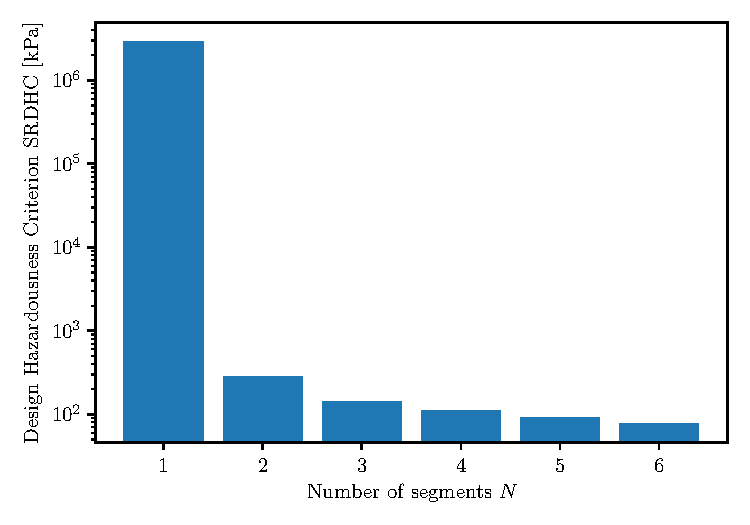
\includegraphics[width=0.5\linewidth]{safetymetric/figures/planar_pcs_design_hazardousness_criterion_discretization/design_hazardousness_criterion_bar_log.pdf}
    \caption{Analysis of the impact of varying the discretization of a planar \gls{PCS} robot on \gls{SRDHC} while keeping the total soft robot length constant at \SI{1}{m}.}
    \label{fig:safetymetric:planar_pcs_design_hazardousness_criterion_discretization}
\end{figure}
\section{Conclusion}
% In this chapter, we first highlighted the absence of a safety metric for soft robots, a gap that prevents the community from quantifying their safety advantages over rigid robot counterparts. This shortfall often results in designs that are ineffective in real-world tasks because they are excessively soft and lack sufficient payload capacity. We then discussed how a quantitative safety metric could be exploited in both design and control applications, ensuring safety without unduly compromising system performance by making the robot overly soft or the motion behavior overly cautious. Finally, we outlined the criteria such a safety metric must meet.
In this chapter, we first underscore the absence of a safety metric for soft robots—a gap that hinders the community from quantifying their safety benefits compared to rigid robots. This shortfall often leads to designs that perform poorly in real-world tasks because they tend to be overly soft and lack sufficient payload capacity. We then explored how a quantitative safety metric could be applied in both design and control contexts, ensuring safety without forcing the robot to be too soft or its motion overly cautious. Finally, we defined the criteria that such a safety metric must satisfy.

% Subsequently, we derived a quantitative safety metric for soft robots while considering the maximum contact pressure experienced during the collision, analog to the existing ISO norms for \glspl{Cobot}~\citep{iso2016collaborative}, as the safety criterion.
% For this the derivation of the safety metric, we rely on existing soft robot dynamic models, such as \gls{PCS}~\citep{renda2018discrete}\footnote{Please refer to Chapter~\ref{chp:background} for a discussion about alternative soft robot models that the safety metric could be based on.} and assume the human to be constrained, which represents the \emph{worst case}~\citep{haddadin2009requirements}.
% The proposed safety metric comes into two flavors: the \gls{SRISC} can be evaluated in closed-form and determines the maximum contact pressure experienced during a soft robot - human collision for a given initial condition, consting of soft robot configuration, velocity and contact geometry, and a given constant (e.g., worst-case) actuation. The \gls{SRISC} is in particular suitable for \emph{safety-aware control} applications.
% However, when designing soft robots, we need to ensure safety within a given operating envelope consisting of infinitely many initial conditions. For this case, we developed the \gls{SRDHC} which determines the maximum \gls{SRISC} for a given specification of operating conditions (e.g., maximum deformation, actuator bounds, configuration-space velocities), in particular across all possible contact geometries.
Next, we derived a quantitative safety metric for soft robots by considering the maximum contact pressure during a collision, analogous to the existing ISO norms for \glspl{Cobot}~\citep{iso2016collaborative}, as our safety criterion. For the derivation, we relied on established soft robot dynamic models, such as \gls{PCS}~\citep{renda2018discrete}\footnote{Please refer to Chapter~\ref{chp:background} for a discussion of alternative soft robot models that could serve as the basis for the safety metric.}, and assumed a constrained human model to represent the \emph{worst case} scenario~\citep{haddadin2009requirements}. The proposed safety metric is offered in two forms: the \gls{SRISC}, which can be computed in closed-form and estimates the maximum contact pressure during a soft robot–human collision given a specific initial condition—comprising the robot’s configuration, velocity, contact geometry, and a predetermined (e.g., worst-case) actuation—and is particularly well-suited for \emph{safety-aware control} applications. In contrast, when designing soft robots, it is necessary to guarantee safety across an operating envelope that encompasses infinitely many initial conditions. For this purpose, we developed the \gls{SRDHC}, which determines the maximum \gls{SRISC} for a given set of operating conditions (e.g., maximum deformation, actuator bounds, configuration-space velocities), especially considering all potential contact geometries.

% Crucially, the proposed safety metric meets all (compulsory) requirements specified in Sec.~\ref{sub:safetymetric:safety_metric_requirements}, as it, for example, accounts for collisions along the entire soft robot body, the assumptions and simplifications taken during the derivation lead to a conservative estimate of the true safety, the computation of the safety metric is tractable as (a) we do not need to the collision dynamics in time but rather have access to the maximum contact force in closed form, (b) part of the computation can be vectorized/parallelized. Furthermore, the safety metric is differentiable - even analytically as our implementation in JAX~\citep{jax2018github} provides gradients via autodifferentiation.
Notably, the proposed safety metric fulfills all mandatory requirements outlined in Sec.~\ref{sub:safetymetric:safety_metric_requirements}. For instance, it takes into account collisions along the entire soft robot body, and the assumptions and simplifications made during its derivation result in a conservative estimate of true safety. Additionally, the metric is computationally tractable because (a) it bypasses the need to simulate collision dynamics over time by providing the maximum contact pressure in closed form, and (b) portions of the computation can be vectorized or parallelized. Moreover, the metric is differentiable—even analytically—since our implementation in JAX~\citep{jax2018github} offers gradients through autodifferentiation.

% Notably, the characterization of the proposed safety metric demonstrated, that the safety of soft robots is not solely determined by material softness, but that instead, also their mass density, actuation, control and operating conditions (e.g., velocity, maximal deformation) play a significant role.
% In particular, feedback gains increase the stiffness of closed-loop system~\cite{della2017controlling, della2023model} therefore also for soft robots, the safety is decreased.
% Furthermore, counter usual intuition, the maximum injury severity is caused neither by collisions at the proximal or distal end, but instead somewhere in between.
% Finally, preliminary research shows that the numerous \glspl{DOF} that soft robot exhibit could be playing a significant role in distributing the contact energy and reducing the maximum local contact pressure.
Notably, the characterization of the proposed safety metric demonstrates that the safety of soft robots is determined not only by their material softness but also by factors such as mass density, actuation, control, and operating conditions (e.g., velocity, maximum deformation). In particular, increased feedback gains raise the stiffness of the closed-loop system~\citep{della2017controlling, della2023model}, thereby reducing safety even for soft robots. Moreover, contrary to common intuition, the maximum injury severity does not occur at either the proximal or distal end, but rather somewhere in between. Finally, preliminary research suggests that the numerous degrees of freedom (\glspl{DOF}) in soft robots may play a significant role in distributing contact energy and reducing the maximum local contact pressure.

% For future work, two critical aspects then emerge: (1) experimentally validating the safety criterion—i.e., measuring the discrepancy between the predicted and actual safety criterion—and (2) establishing appropriate thresholds~\citep{iso2016collaborative, behrens2022statistical} for the safety criterion (i.e., acceptable injury risk) to ensure safety in human-centric environments. Here, analog the existing literature on rigid robots~\citep{yamada1997evaluation, muttray2014collaborative, behrens2022statistical}, empirical biomechanical studies could play a crucial role in this process.
% It is important to note that safety requirements may differ significantly depending on the specific robotic application and task. For instance, a soft robot designed as a children's toy must adhere to much stricter safety standards than one used for industrial refueling. Understanding such varying requirements is crucial to ensuring safe and effective performance. 
Looking ahead, two key aspects emerge for future work: (1) the experimental validation of the safety criterion—i.e., quantifying the discrepancy between predicted and actual safety—and (2) the establishment of appropriate thresholds~\citep{iso2016collaborative, behrens2022statistical} for the safety criterion (in terms of acceptable injury risk) to ensure safety in human-centric environments. Drawing inspiration from existing literature on rigid robots~\citep{yamada1997evaluation, muttray2014collaborative, behrens2022statistical}, empirical biomechanical studies could play a crucial role in this process. It is also essential to recognize that safety requirements may vary considerably depending on the specific robotic application and task. For example, a soft robot designed as a children’s toy must comply with much stricter safety standards than one intended for industrial refueling. Understanding these differences is key to achieving safe and effective performance.

% Furthermore, the safety metric itself can be extended and improved. For example, specializing in safety metrics for different soft robot modeling techniques, such as FEM-based and geometric strain-based approaches, will enable more accurate risk assessments tailored to specific designs. Extending these metrics to closed-chain robots, locomotors, and wearable systems will further solidify safety evaluation frameworks across diverse robotic applications.
Furthermore, the safety metric itself can be extended and refined. By developing specialized metrics tailored to different soft robot modeling techniques—such as \gls{FEM}- or \gls{GVS}-based approaches—more accurate risk assessments can be achieved for specific designs. Extending these metrics to closed-chain robots, locomotors, and wearable systems will further strengthen safety evaluation frameworks across a diverse range of robotic applications.

% Finally moving to applications, we find it crucial to develop develop design and control concepts that can exploit the proposed safety metric.
% First considering \emph{safety-aware design}, a critical next step involves identifying which design parameters most significantly affect safety in different types of actuation, such as tendon-driven and pneumatically actuated soft robots. Mapping out these dependencies will provide actionable insights for designers seeking to enhance safety.
% Furthermore, we propose in Appendix~\ref{chp:apx:holisticcodesign} a strategy for co-optimizing the safety of soft robots via co-design~\citep{zardini2023co, spielberg2019learning, wang2024diffusebot, navez2024contributions}, which will allow to explicitly formalize and quantify the tradeoff between safety and performance in soft robotics.
Finally, with regard to practical applications, it is vital to develop design and control strategies that take full advantage of the proposed safety metric. In the context of\emph{safety-aware design}, a crucial next step is to identify which design parameters most significantly impact safety for various actuation types, such as tendon-driven versus pneumatically actuated soft robots. Mapping these dependencies will provide designers with actionable insights to enhance safety. Additionally, as outlined in Appendix~\ref{chp:apx:holisticcodesign}, we propose a holistic co-design strategy for optimizing the safety of soft robots~\citep{zardini2023co, spielberg2019learning, wang2024diffusebot, navez2024contributions}, which will enable the explicit formalization and quantification of the trade-off between safety and performance in soft robotics.
% On the other hand, \emph{safety-aware control} could be achieved via \gls{MPC} or \glspl{CBF}~\citep{ames2016control, ferraguti2020control}, which would enable us to push the performance (e.g., speed~\citep{haggerty2023control}) as much as possible while still guaranteeing safety in all scenarios.
Additionally, \emph{safety-aware control} can be implemented, for example, using \gls{MPC} or \glspl{CBF}~\citep{ames2016control, ferraguti2020control}, enabling us to maximize performance, such as the motion speed~\citep{haggerty2023control}, while ensuring safety in all scenarios.

% \section{Design of Safe Soft Robots}
% \begin{itemize}
%     \item Based on the insights gained in Section~\ref{sec:safety_metric}, give \emph{simple} insights how safe designs can be achieved.
%     \item Stiffness of the soft robot design (i.e., not just of the material) should be reduced, particularly close to the base/proximal end.
%     \item Reflected mass (e.g., material density \& volume) should be reduced, in particular close to the tip/distal end.
%     \item Guidelines for establishing safe controllers.
%     \item Specifically, explain how the combination of robot stiffness and the proportional control gains impacts the design hazardousness.
%     \item However, we stress that \emph{simple} guidelines that guarantee a specific safety level cannot be (easily) expressed. Therefore, we require a co-design methodology that takes into account the safety metric.
% \end{itemize}
